% !TEX root = master_thesis.tex
\chapter{Event selection}
\label{chap:events}
The determination of polarization observables needs to be performed for particular reactions (cf. chapter \ref{chap:intro}), such as the photoproduction of e.g. a single $\eta'$ meson. However, the recorded events  contain data from the decay products of several possible final states in addition to combinatorial background. Thus, event candidates for the desired reaction have to be extracted before they are considered for further analysis. Table \ref{tab:etap} shows the five most probable decay modes of the $\eta$ and $\eta'$ meson. Three decay channels of the $\eta'$ contain final states which only contain photons and are thus reliably measurable with the CBELSA/TAPS experiment. Only the $\eta'\to\gamma\gamma$ decay channel was considered for further analysis; the $\omega\gamma$ channel provides negligible statistics and considering the acceptance of detecting six photons in the final state, the expected yield of the $\eta'\to\gamma\gamma$ decays should be roughly equal to the $\eta'\to\pi^0\pi^0\eta\to6\gamma$ final state \cite{farahmsc}. Offering a simpler, three-particle final state, the $\eta'\to\gamma\gamma$ channel was then favored in the course of this thesis. The $\eta$ meson on the other hand decays dominantly into two photons making it the preferred decay channel when determining the beam asymmetry.
\begin{table}[htbp]
	\centering
	\begin{tabular}{cc|cc}
		\toprule
		\multicolumn{2}{c|}{$\eta$}&\multicolumn{2}{c}{$\eta'$}\\
		\hline
		Decay mode&Branching ratio&Decay mode&Branching ratio\\
		\hline
		$\gamma\gamma$&39.36\%&$\pi^+\pi^-\eta$&42.6\%\\
		$3\pi^0\gamma$$(\to6\gamma$) &32.57\% (31.43\%)&$\rho^0\gamma(\to\pi^+\pi^-\gamma)$ &28.9\% (28.9\%)\\
	$\pi^+\pi^-\pi^0$ & $22.02\%$ &$\pi^0\pi^0\eta(\to6\gamma$) & 22.8\% (8.8\%)\\
		$\pi^+\pi^-\gamma$&$4.28\%$&$\omega\gamma(\to \pi^+\pi^-\pi^0\gamma/\pi^0\gamma\gamma)$&2.52\% (2.2\%/0.21\%)\\
	$e^+e^-\gamma$&0.69\%&$\gamma\gamma$&2.3\%\\

		\bottomrule
	\end{tabular}
\caption{The five most probable decay modes of the $\eta$ and $\eta'$ meson. The most probable further decay with according branching ratio is shown in brackets.\cite{pdg}}
\label{tab:etap}
\end{table}

\noindent The process of \emph{event selection} for the reaction $\gamma p \to p\eta'\to p\gamma\gamma$ is outlined in the following chapter. Note that in this thesis the event selection of the $p\eta\to p\gamma\gamma$ final state was already performed by \textsc{F. Afzal} \cite{farahphd} and the selected data are only used to determine the beam asymmetry via \textsc{Bayesian} statistics, see section \ref{sec:sigmaeta}. Nevertheless, a short summary of the according event selection is given at the end of this chapter, for a more detailed review, see reference \cite{farahphd}.
\section{Reconstruction of events}
In order to proceed with the analysis the initial and final state particles' four momenta $p$ need to be known for every event. The employed calorimeters are capable of delivering this information; the tagger setup allows mapping fiber or bar hits to a beam photon energy. Each beam photon is assigned the mean energy $E_\gamma$ over all tagger hits. Since the target protons are at rest, these informations suffice to determine the initial state four momenta
\begin{align}
	p_{\gamma,\text{ beam}}=\begin{pmatrix}
		E_\gamma\\0\\0\\E_\gamma 
	\end{pmatrix}
&&
 p_p=\begin{pmatrix}
	m_p\\0\\0\\0\\
\end{pmatrix} .
\end{align}
Once a final state particle passes through sensitive detector material it will deposit a certain amount of energy by interacting with it. In most cases this will result in an electromagnetic shower that will span over several detector elements. Timely and spatially correlated showers are grouped to \emph{clusters} using clusterfinding algorithms, depending on the hit detector. As a next step, clusters are scanned for local energy deposition maxima, which mark a \emph{particle energy deposition} (PED), corresponding to a single particle. Clusters hereby may have more than one PED. The assigned energy $E_i$ for each particle $i$ is the sum of all energy depostions belonging to a PED. Furthermore, a weighted average over all crystal hits will give a polar angle $\theta_i$ and azimuthal angle $\phi_i$ \cite{angles1}. If a particle only hits the inner detector both angles can be calculated from several timely correlated fiber hits \cite{angles2}. Finally, all informations are combined to form the four momentum of a final state particle, assuming it is massless
\begin{equation}
		p_i=\begin{pmatrix}
		E_i\\E_i\cos\phi_i\sin\theta_i\\E_i\sin\phi_i\sin\theta_i\\E_i\cos\theta_i 
	\end{pmatrix}.
\end{equation}
This four momentum is wrong if the detected particle is a proton since it has non vanishing mass. However, the protons energy information is not a reliable quantity since they often leave the calorimeters without depositing their entire energy. The assigned four momenta are thus only used to access their angular information. In addition to energy and momentum the CBELSA/TAPS setup allows to assign time and charge information for all particles hitting the inner, forward or MiniTAPS detector\footnote{Actually, the experiment has been upgraded to provide time information for particles hitting the Crystal Barrel as well in 2017 \cite{urban}}. 
\section{Preselection and charge cut}
Since the polarization degree can only be evaluated reliably up to \SI{1800}{\mega\eV} and the production threshold for $\eta'$ mesons is $E_\gamma=\SI{1447}{\mega\eV}$ \cite{pdg}, the beam photon energy range was restricted to \SIrange{1400}{1800}{\mega\eV} from the very beginning. The measured events are then generally classified depending on the number of PEDs. If three final state particles are measured, they are referred to as 3PED events. Low energy protons however may either be only detected in the scintillators of the inner, forward or MiniTAPS detector -- giving directional information from scintillator bar hits only (2.5 PED) -- or lost entirely (2 PED). Only 3PED events were analyzed since the additional background contributions from 2PED and 2.5PED events exceeded the additional signal contributions. It is worth noting that 3PED events are significantly dominant for $\eta'\to\gamma\gamma$ reactions; the production threshold for $\eta'$ mesons at $E_\gamma=\SI{1447}{\mega\eV}$ \cite{pdg} is so high energetic that the recoil proton will likely be detected. Figure \ref{fig:PEDs} shows the distribution of the different event classes for $\eta'\to\gamma\gamma$ production in \textsc{Monte Carlo} data, with a clear preference towards 3PED events.
\begin{figure}[htbp]
	\centering
	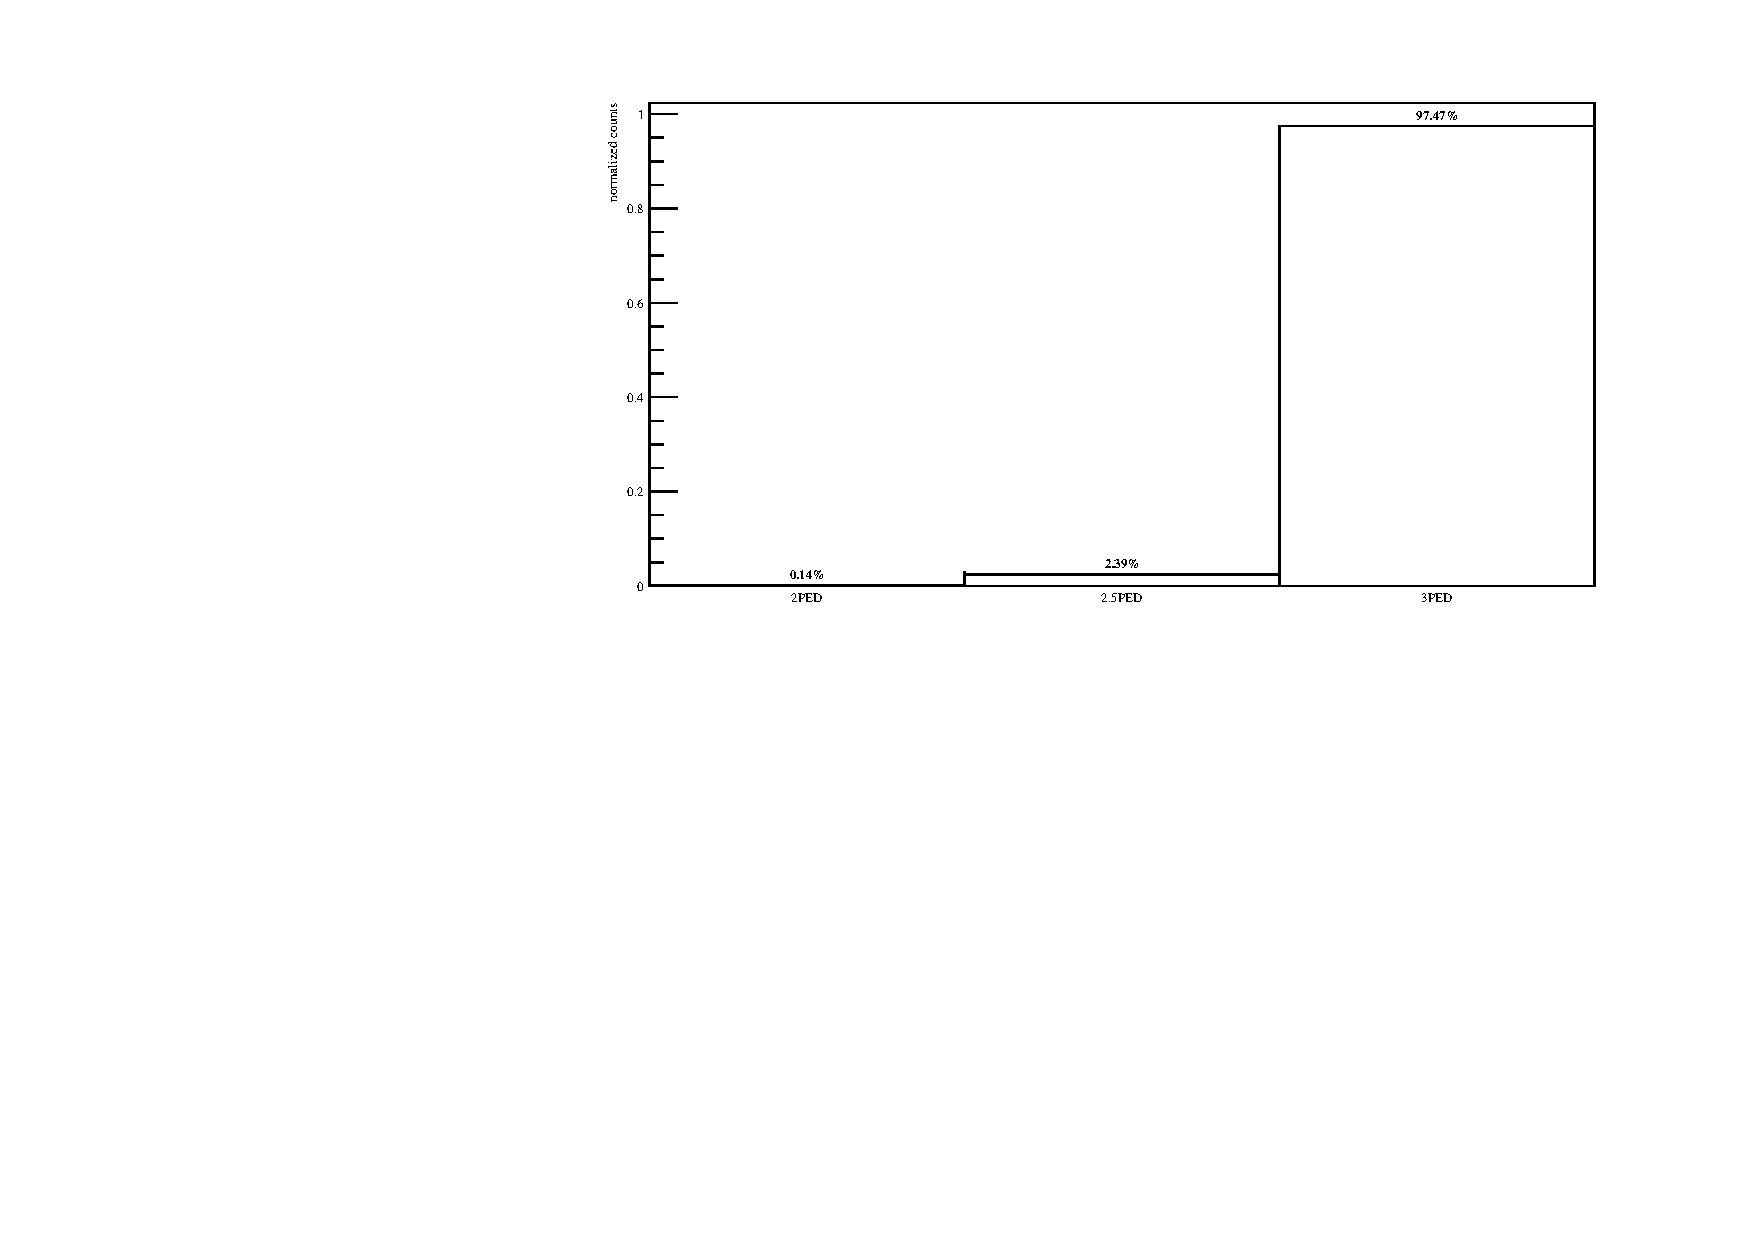
\includegraphics[width=\linewidth]{../figs/hydrogen/PEDs.pdf}
	\caption{Distribution of event classes in $\eta'\to\gamma\gamma$ production}
	\label{fig:PEDs}
\end{figure}
To further improve the signal to background ratio, the charge information of the final state particles was utilized in the next step. In particular, to select  $\eta'\to\gamma\gamma$ reactions, one charged and two uncharged particles in the final state were demanded. 

\section{Time of particles}
\label{sec:time}
Due to its high count rate the tagging system (see section \ref{subsec:tag}) will not only record beam photons which produce the detectable final state particles, but also several uncorrelated ones. To select only beam photons which will induce a photoproduction process the time information of the detected particles is used. It is shown in figure \ref{fig:time} for all particles involved in 2.5PED and 3PED events of $\eta'$ photoproduction. 
\begin{figure}[htbp]
	\centering
	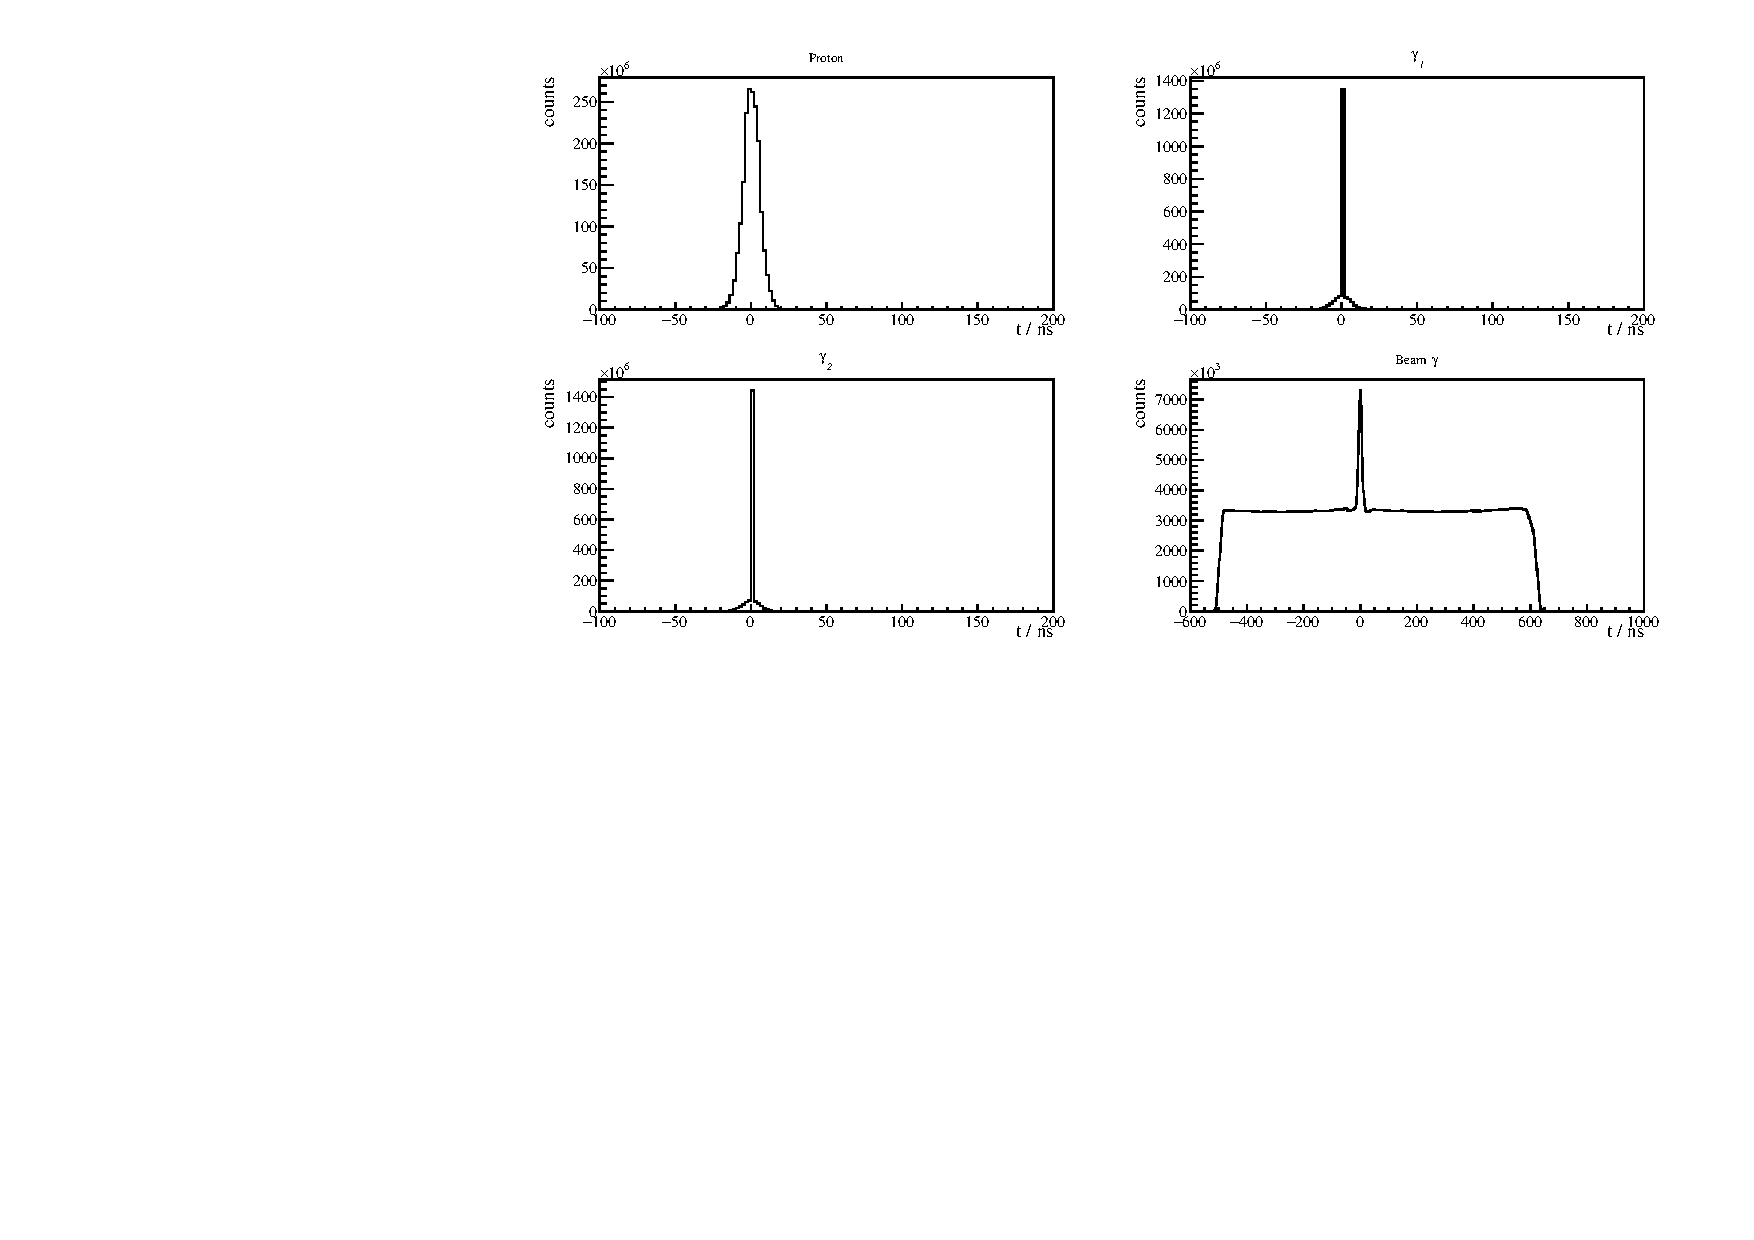
\includegraphics[width=\linewidth]{../figs/hydrogen/time/times.pdf}
	\caption{Time information of all final state particles and the beam photon for 3PED $\eta'$ production}
	\label{fig:time}
\end{figure} 
In all cases prompt peaks centered around \SI{0}{\nano\s} (the trigger time) are visible. Since the final state photons move with velocity $c$ their timing information does not underlie fluctuations, as is the case for the final state proton on the contrary. The tagged, uncorrelated beam photons are visible as flat background underneath the prompt peak in the time of the beam photon. Naturally, only coincident events may be referred to  as $\gamma p\to p\eta'$ reaction candidates for the further analysis and thus only events with time information of at least one final state particle are kept. Photons need to be detected in the MiniTAPS or forward
detector to acquire time information. To determine coincidence it is convenient to define the \emph{reaction time} 
\begin{equation}
	t_\text{reaction}=\begin{cases}
		t_\text{beam}-t_\text{meson} & \text{ meson time exists}\\
		t_\text{beam}-t_\text{recoil} & \text{ meson time does not exist},
	\end{cases}
\end{equation}
where the meson time $t_\text{meson}$ is appointed either the averaged time of both decay photons or the time of a single photon if only one photon has time information. $t_\text{beam}$ and $t_\text{recoil}$ are the time of the beam photon and recoil proton, respectively. Figure \ref{fig:time_r} shows the reaction time for 2.5PED and 3PED events; a clear prompt peak centred at 0 is visible, the colored area indicates the chosen range of $t_\text{reaction}\in[-8,5]\si{\nano\s}$. However, this cut still contains random time background underneath the prompt peak. This may be accounted for by \emph{sideband substraction}, assuming the background is flat. All events residing in the prompt peak with $t_r\in[-8,5]\si{\nano\s}$ will be assigned a weight of $w_p=+1$ while sideband events with $t_r\in[-200,-100]\si{\nano\s}\lor t_r\in[100,200]\si{\nano\s}$ will be assigned a weight of $w_s=-\frac{13}{200}$. Events with $t_r$ neither in the sideband nor in the prompt peak get assigned a weight of $w=0$. Any histogram $N$ that is filled in the following will then consist of prompt peak events $N_\text{prompt}$ and sideband events $N_\text{sideband}$ $$N=N_\text{prompt}+w_s\cdot N_\text{sideband},$$ such that the random time background underneath the prompt peak is substracted. In addition, the time difference between meson and proton and between the two photons is demanded to be within $[-10,10]\si{\nano\s}$. All described cuts to the data, including the sideband substraction are referred to as the \emph{time cut} in the following.

\begin{figure}[htbp]
	\centering
	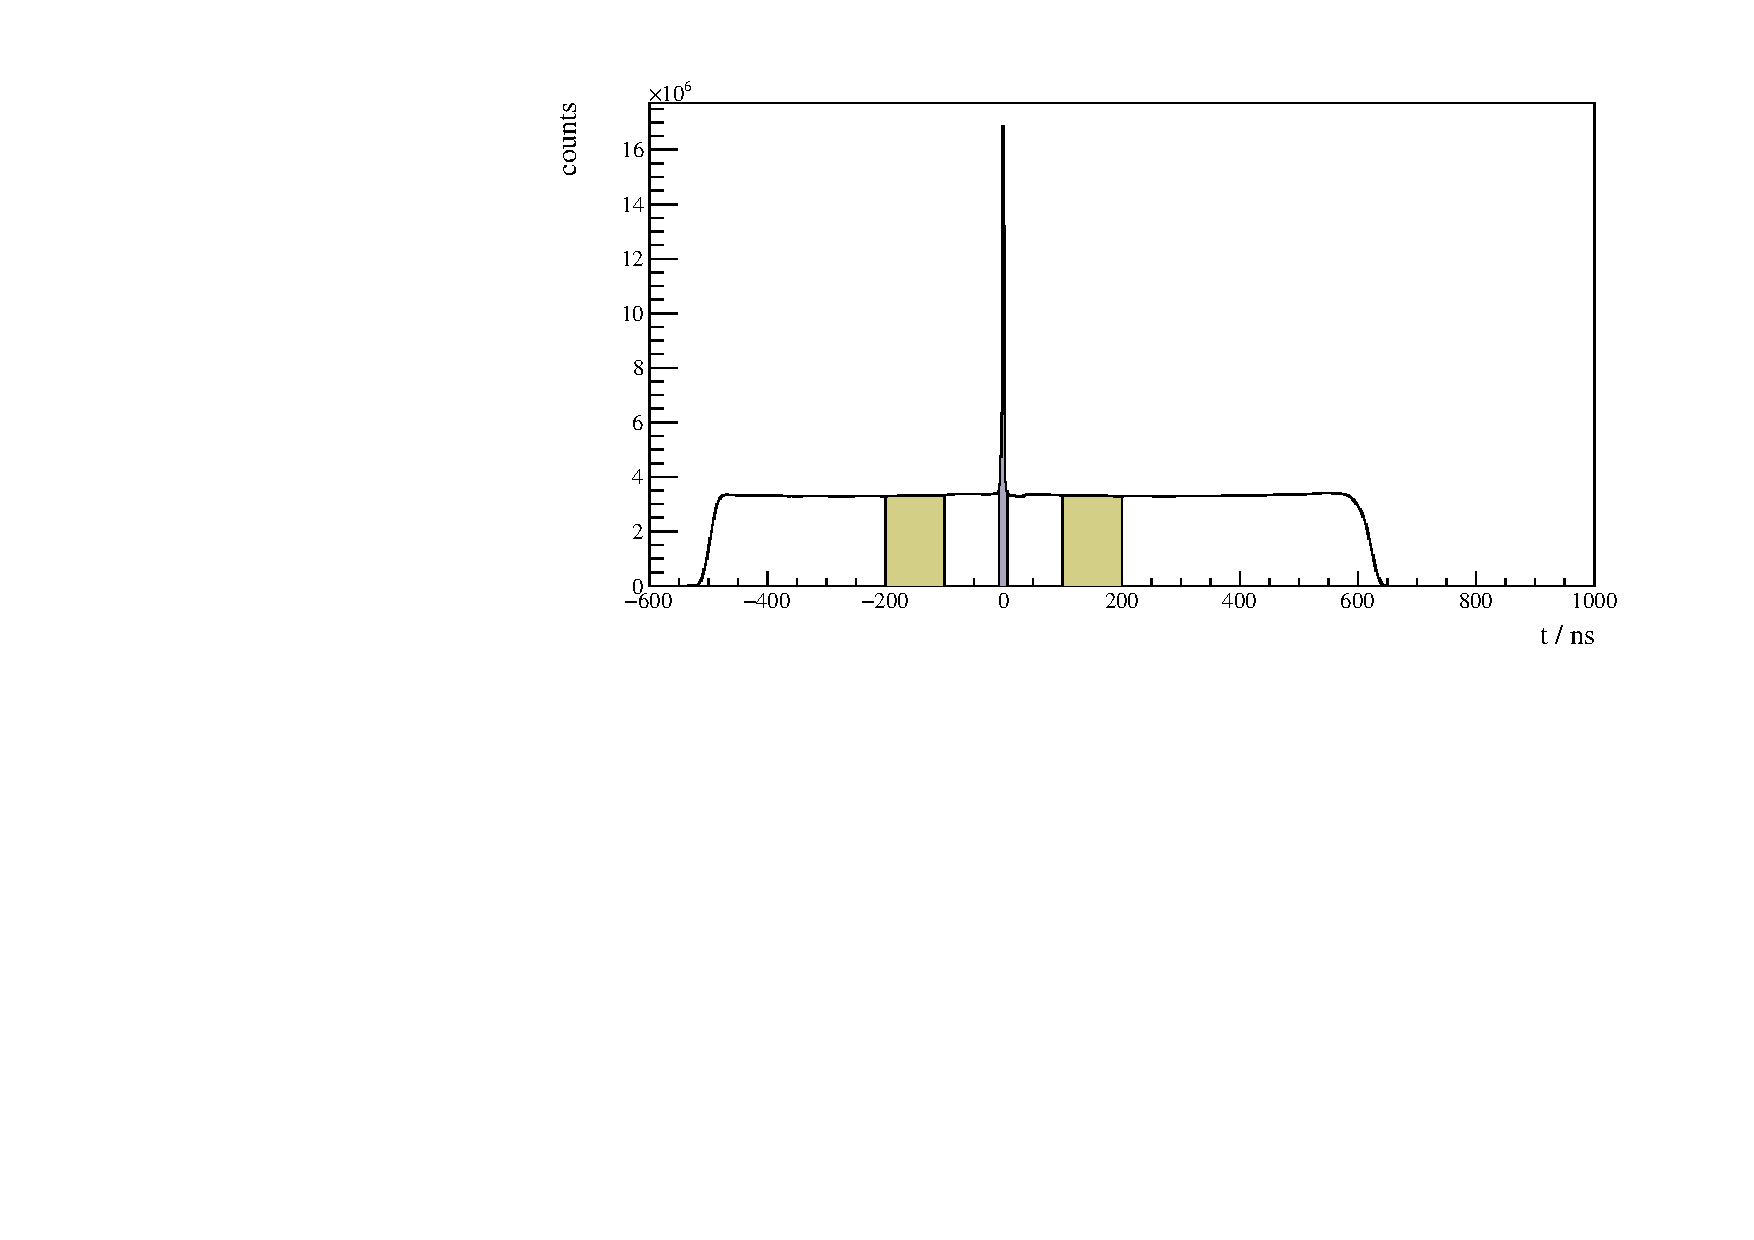
\includegraphics[width=\linewidth]{../figs/hydrogen/time/reaction_time.pdf}
	\caption{Reaction time $t_r$ for 3PED and 2.5PED $\eta'$ production. The yellow region indicate the sidebands while the purple colored interval is the selected prompt peak.}
	\label{fig:time_r}
\end{figure} 

\section{Kinematic constraints}
Up to now mainly combinatorial background caused by the amount of beam photon candidates was discussed. However one can derive kinematical constraints from energy and momentum conservation to exclusively select the desired reaction. The derivation is discussed first, followed by the determination of the derived cut conditions.
\subsection{Derivation of cut conditions}
Let $p_\text{beam}$ and $p_p$ be the four momenta of the initial state beam photon and proton, respectively. Then it holds \begin{equation}
	p_\text{beam}+p_p=p_\text{recoil}+p_\text{meson},
	\label{eq:kin}
\end{equation}
with $p_\text{recoil}$ being the momentum of the recoiling proton and $p_\text{meson}$ the meson momentum.
\subsubsection{Coplanarity}
In the initial state there is vanishing transverse momentum $p_{xy}$ since the target protons are at rest and the beam photon impinges in $z$-direction. Naturally, this transverse momentum has to vanish in the final state as well, such that \begin{equation}
	\mathcal{P}_{xy} \left[p_\text{recoil}+p_\text{meson}\right]=0,
	\label{eq:copl}
\end{equation}
where $\mathcal{P}_{xy}$ is the projection operator to the transverse plane. Equation \eqref{eq:copl} is valid if and only if meson and proton lie back to back (coplanar) in the $x$-$y$ plane, which is quantified by the difference of their azimuthal angles $\phi_\text{meson}$ and $\phi_\text{recoil}$ being $\SI{180}{\degree}$ in the laboratory-frame
\begin{equation}
	\Delta\phi:=\phi_\text{meson}^\text{LAB}-\phi_\text{recoil}^\text{LAB}\overset{!}{=}\SI{180}{\degree}.
\end{equation}
\subsubsection{Polar angle difference}
If all initial and final state momenta are measured, the reaction described by equation \eqref{eq:kin} is \emph{overdetermined}, such that one final state particle can be treated as a "missing particle" $X$ with momentum $p_X$: 
\begin{equation}
	p_X=p_\text{beam}+p_p-p_\text{meson}.
	\label{eq:polangle}
\end{equation}
One can then use the polar angle difference
\begin{equation}
\Delta\theta:=\theta_{p_X}^\text{LAB}-\theta_{p_\text{recoil}}^\text{LAB}\overset{!}{=}0
\label{eq:polarangle}	
\end{equation}
as a further constraint to the data.
\subsubsection{Missing mass}
The previously described angular cuts are only applicable if all final state particles have been detected. Independently of the detection of the recoil proton the mass of the missing particle $m_X^2=p_X^2$ can be determined and compared with the proton mass of $m_p=\SI{938.27}{\mega\eV}$ \cite{pdg}. From Eq. \eqref{eq:polangle} it follows that \begin{equation}
	m_X=\sqrt{(E_\gamma+m_p-E_\text{meson})^2-p_{x,\text{meson}}^2-p_{y,\text{meson}}^2-(E_\gamma-p_{z,\text{meson}})^2}.
	\label{eq:mism}
\end{equation}
\subsubsection{Invariant mass}
The measurement of the invariant mass of the two final state photons does also not require the measurement of the recoil proton. The knowledge of both decay photon four-momenta $p_{\gamma_1}$ and $p_{\gamma_2}$ suffices, since \begin{equation}
	m_\text{meson}=\sqrt{p_\text{meson}^2}=\sqrt{(p_{\gamma_1}+p_{\gamma_2})^2}=\sqrt{2E_{\gamma_1}E_{\gamma_2}(1-\cos\alpha_{\gamma_1\gamma_2})},
\label{eq:invm}
\end{equation}
where $E_{\gamma_i}$ are the measured photon energies and $\alpha_{\gamma_1\gamma_2}$ is the angle between the two decay photon momenta. To select only $\eta'$ candidates $m_\text{meson}=m_{\eta'}=\SI{957.78}{\mega\eV}$ is demanded. Remarkably, the cut on the invariant mass of the final state photons is the only one to uniquely select $\eta'$ production candidates so far. All other cuts apply similarly to arbitrary meson photoproduction.
\subsection{Determination of cut ranges}
The constraints described in the previous section must not be understood as strict equalities, cf. equations \eqref{eq:copl},\eqref{eq:polarangle},\eqref{eq:mism} and \eqref{eq:invm}. The quantities of interest will rather describe distributions around the desired value, such that confidence intervals may be extracted by fitting to said distributions. This is done iteratively:

Let $\mathcal{C}^\chi_{\mathcal{I}}$ be the cut operator that restrains the data $\mathcal{D}$ such that the (generic) cut variable $$\chi\in\{\Delta\theta,\Delta\phi,m_X,m_\text{meson}\}$$ lies in the interval $\mathcal{I}\subseteq\mathbb{R}$, such that 
\begin{equation}
	\mathcal{C}_{\mathcal{I}}^\chi:\mathcal{D}\mapsto\mathcal{D}_{\chi\in\mathcal{I}} .
\end{equation}
	 After a first inspection of the data, initial guesses for the intervals $\mathcal{I},\mathcal{J},\mathcal{K},\mathcal{L}$ corresponding to the quantities $\Delta\theta,\Delta\phi,m_X,m_\text{meson}$, respectively, are made.
	Having established estimates for the cut ranges, new ones are estimated by investigating the distribution of one cut variable obtained from the data while all other cut variables are constrained to the previously determined intervals. For example 
	$$\Delta\theta\left(\mathcal{C}_\mathcal{J}^{\Delta\phi}\mathcal{C}_\mathcal{K}^{m_X}\mathcal{C}_\mathcal{L}^{m_\text{meson}}\mathcal{D}\right)\sim \text{normal}(\mu,\sigma),$$
	where $\mu\approx0$. This is done (with some adjustments to the fit function) for each cut variable. The parameters of the gaussian are determined from a $\chi^2$ fit and used to assign new cut ranges. Simultaneously, Monte-Carlo (MC) data of relevant final states are fitted to match the measured values bin-wise. This is done on the one hand to check consistency between measured and MC data and on the other hand used to determine contributing background reactions. First, all mesonic final states that decay into two photons are considered, i.e. $p\pi^0,p\eta,p\eta'$, since the according peaks in the invariant mass spectrum will be visible. Also, a peak at the mass of the $\omega$ (vector)-meson $m_\omega$ will be visible; this stems from photoproduction reactions $p\omega\to p\pi^0\gamma\to p3\gamma$ where one low energetic final state photon is lost, such that the reconstructed invariant mass still estimates the $\omega$ mass. Further, one should investigate the impact of neutral final states, where some of the final state photons may get lost during reconstruction, as can be observed for $p2\pi^0,p\pi^0\eta,p3\pi^0$ \footnote{all mesons $m$ decaying into two photons is implied: $m\to\gamma\gamma \forall m$} production. Lastly, possible misidentifiaction of charged particles in very frequent reactions which then mimic a $p\gamma\gamma$ final state are examined, such as $p\pi^+\pi^-$ and $n\pi^+$. Table \ref{tab:mc} lists all employed MC reactions and their respective final state particles, as well as a short explanation why the particular reaction was included in the fit.
	
	\begin{table}[htbp]
		\begin{tabular}{ccc}
			\toprule
			Photoproduction reaction &Final state particles&Explanation\\
			\hline
			$p\pi^0$ & $p\gamma\gamma$&prominent peak in the invariant mass spectrum \\
			$p\eta$ & $p\gamma\gamma$& \\
			$p\omega$ & $p\pi^0\gamma\to p3\gamma$& \\
			$p\eta'$ & $p\gamma\gamma$&\\
			$p2\pi^0$ & $p4\gamma$&lost photons cause a "3-particle" final state\\
			$p\pi^0\eta$ & $p4\gamma$&\\
			$p3\pi^0$ & $p6\gamma$&\\
			$p\pi^+\pi^-$ &$p\pi^+\pi^-$&misidentification of charged particles, large $\sigma$\\
			$n\pi^+$ &$n\pi^+$&\\
			\bottomrule
		\end{tabular}
	\caption{Examined MC reactions that were used in sum for the fit}
	\label{tab:mc}
	\end{table}
	
	 Since the invariant mass spectrum features rich contributions from many final states, it is difficult to describe by a (sum of) gaussian function(s), especially considering the background contributions. Thus, for the invariant mass the cut ranges are obtained from gaussian fits to the scaled MC data of the $\eta'$ final state. Table \ref{tab:cuts} shows which fit function and cut range was used for each cut variable. In addition, it shows if the cut ranges were determined from MC or measured data.
	\begin{table}[htbp]
		\centering
		\begin{tabular}{cccc}
			\toprule
			cut variable & fit function & interval range & obtained from\\
			\hline
			$\Delta\theta$&\textsc{Gauss}&$\mathcal{I}'=[\mu-3\sigma,\mu+3\sigma]$&data points\\
			$\Delta\phi$&\textsc{Gauss}&$\mathcal{J}'=[\mu-3\sigma,\mu+3\sigma]$&data points\\
			$m_X$&\textsc{Novosibirsk} \cite{nov}&$\mathcal{K}'=[\mu-2\sigma,\mu+2\sigma]$&data points\\
			$m_\text{meson}$&\textsc{Gauss}&$\mathcal{L}'=[\mu-2\sigma,\mu+2\sigma]$&MC data\\
			
			\bottomrule
		\end{tabular}
		\caption{Fit functions and cut ranges for each kinematic variable}
		\label{tab:cuts}
	\end{table}
The newly obtained intervals $\mathcal{I}',\mathcal{J}',\mathcal{K}',\mathcal{L}'$ serve again as input for the previous step. This is repeated until a certain convergence is reached, which is usually the case after two or three iterations.
 Since the cut ranges may vary depending on beam energy and meson direction, they are determined in bins of the beam energy and the polar angle of the meson in the center of mass system (CMS) $$(E_\gamma,\cos\theta_{\eta'}^\text{CMS}) \footnote{If not otherwise specified, from now on $\cos\theta=\cos\theta_{\eta'}^\text{CMS}$}.$$ Respecting the $\eta'$ final state statistics, a binning of $\Delta E_\gamma=\SI{100}{\mega\eV}$ and $\Delta\cos\theta=1/3$ was chosen, spanning the energy range of \SIrange{1500}{1800}{\mega\eV}. The theoretically accessible lower limit in the beam energy is provided by the production threshold of $\eta' $ mesons at \SI{1447}{\mega\eV} \cite{pdg}. Yet, the binning has to comply with the upper beam energy limit which is bound from above \footnote{Significantly beyond the coherent edge, the systematic error for the beam polarization  degree gets too large ($>10\%$) while at the same time the polarization degree decreases rapidly ($<10\%$)} by the position of the coherent edge of the beamtime. It is given by \SI{1700}{\mega\eV} and \SI{1800}{\mega\eV} for the July/August and September/October beam times, respectively. If one were to include the production threshold into the analyzed range using the same binning, more background than $\eta'$ events are collected from the beam energy bin \SIrange{1400}{1500}{\mega\eV} because the cross section $\sigma(\gamma p \to p\eta')$ slowly rises to its maximum in this range \cite{etap_cs}, hence the chosen binning starts at \SI{1500}{MeV}.
 
 \subsubsection{Coplanarity}
 Figure \ref{fig:copl} shows the coplanarity spectra for the energy bin $\SI{1500}{\mega\eV}\leq E_\gamma<\SI{1600}{\mega\eV}$ and all angular bins. The data points are visualized by the open circles with error bars, while the black solid histogram is a fit of $\eta'\to\gamma\gamma$ MC. As expected, a clear peak is visible at $\Delta\phi=\SI{180}{\degree}$, which shows only slight dependence on beam energy and meson direction. A $3\sigma$ interval obtained from a gaussian fit is indicated by the dashed red lines. Note that only MC spectra of the $\eta'$ final state were fitted to the data since the coplanarity gives little reference points for a correct estimation of other final states that may contribute. 
   \begin{figure}[htbp]
 	\centering
 	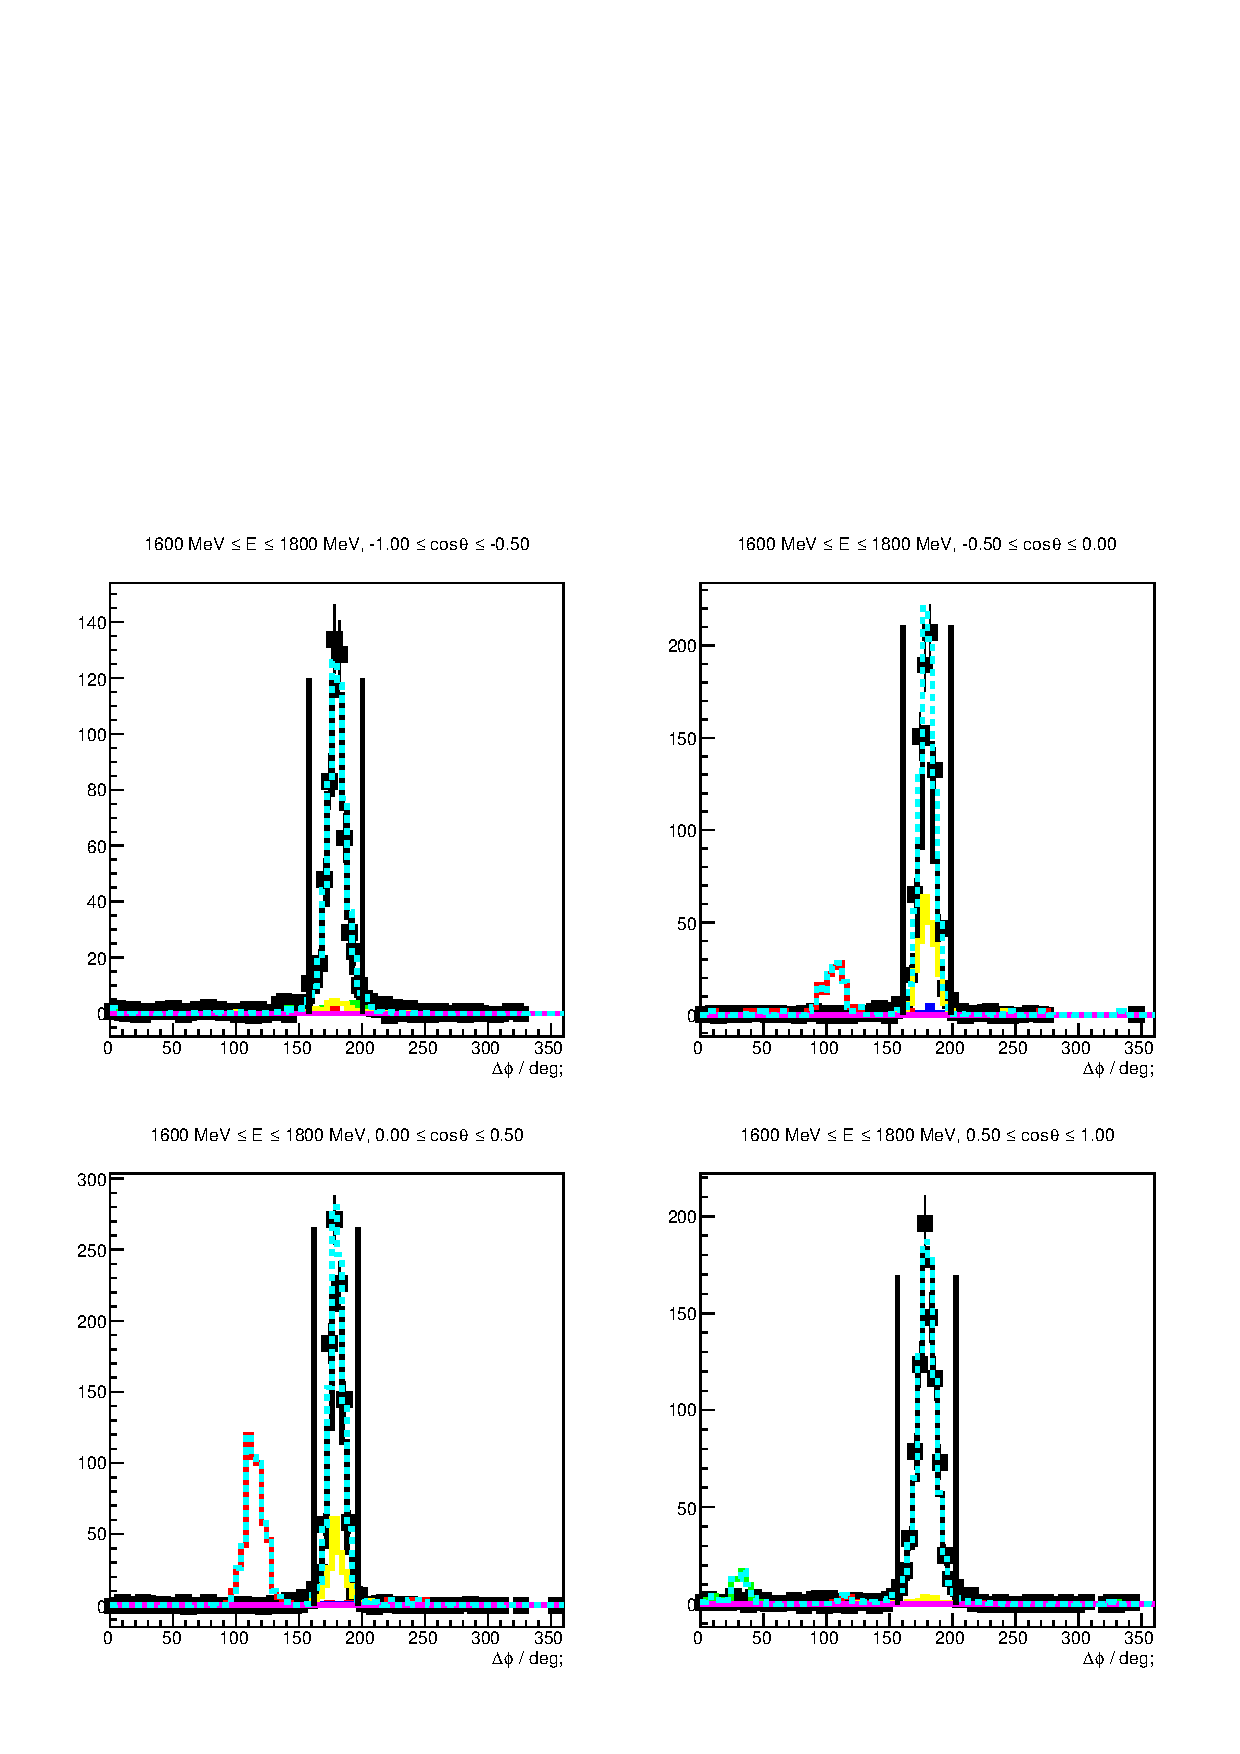
\includegraphics[width=\linewidth]{../figs/hydrogen/bin_cuts/phicut_ebin1.pdf}
 	\caption{Coplanarity of the $p\eta'$ final state with all other cuts applied for the energy bin $\SI{1500}{\mega\eV}\leq E_\gamma<\SI{1600}{\mega\eV}$. The vertical dashed lines show the cut ranges obtained from a gaussian fit to the data (open circles). The solid black histograms represent fitted MC data of $\eta'\to\gamma\gamma$}
 	\label{fig:copl}
 \end{figure}
 \subsubsection{Polar angle difference}
 Since the meson direction correlates with the detector(s) that the final state photons hit, the polar angle difference depicts a clear directional dependence as can be seen in figure \ref{fig:pol} for the energy bin $\SI{1500}{\mega\eV}\leq E_\gamma<\SI{1600}{\mega\eV}$ and all angular bins. In the CMS frame, meson and proton are emitted back to back. Thus, if the meson is emitted in backward direction ($\cos\theta\sim -1$), the proton will be detected either in the forward or MiniTAPS detector, which have a better angular resolution than the Crystal Barrel calorimeter, leading to narrower distributions of $\Delta\theta$. The determined cut ranges are $3\sigma$ intervals obtained from a gaussian fit to the data and are indicated by the red dashed lines. As before, no other than $\eta'$ MC are fitted to the spectra.
  \begin{figure}[htbp]
 	\centering
 	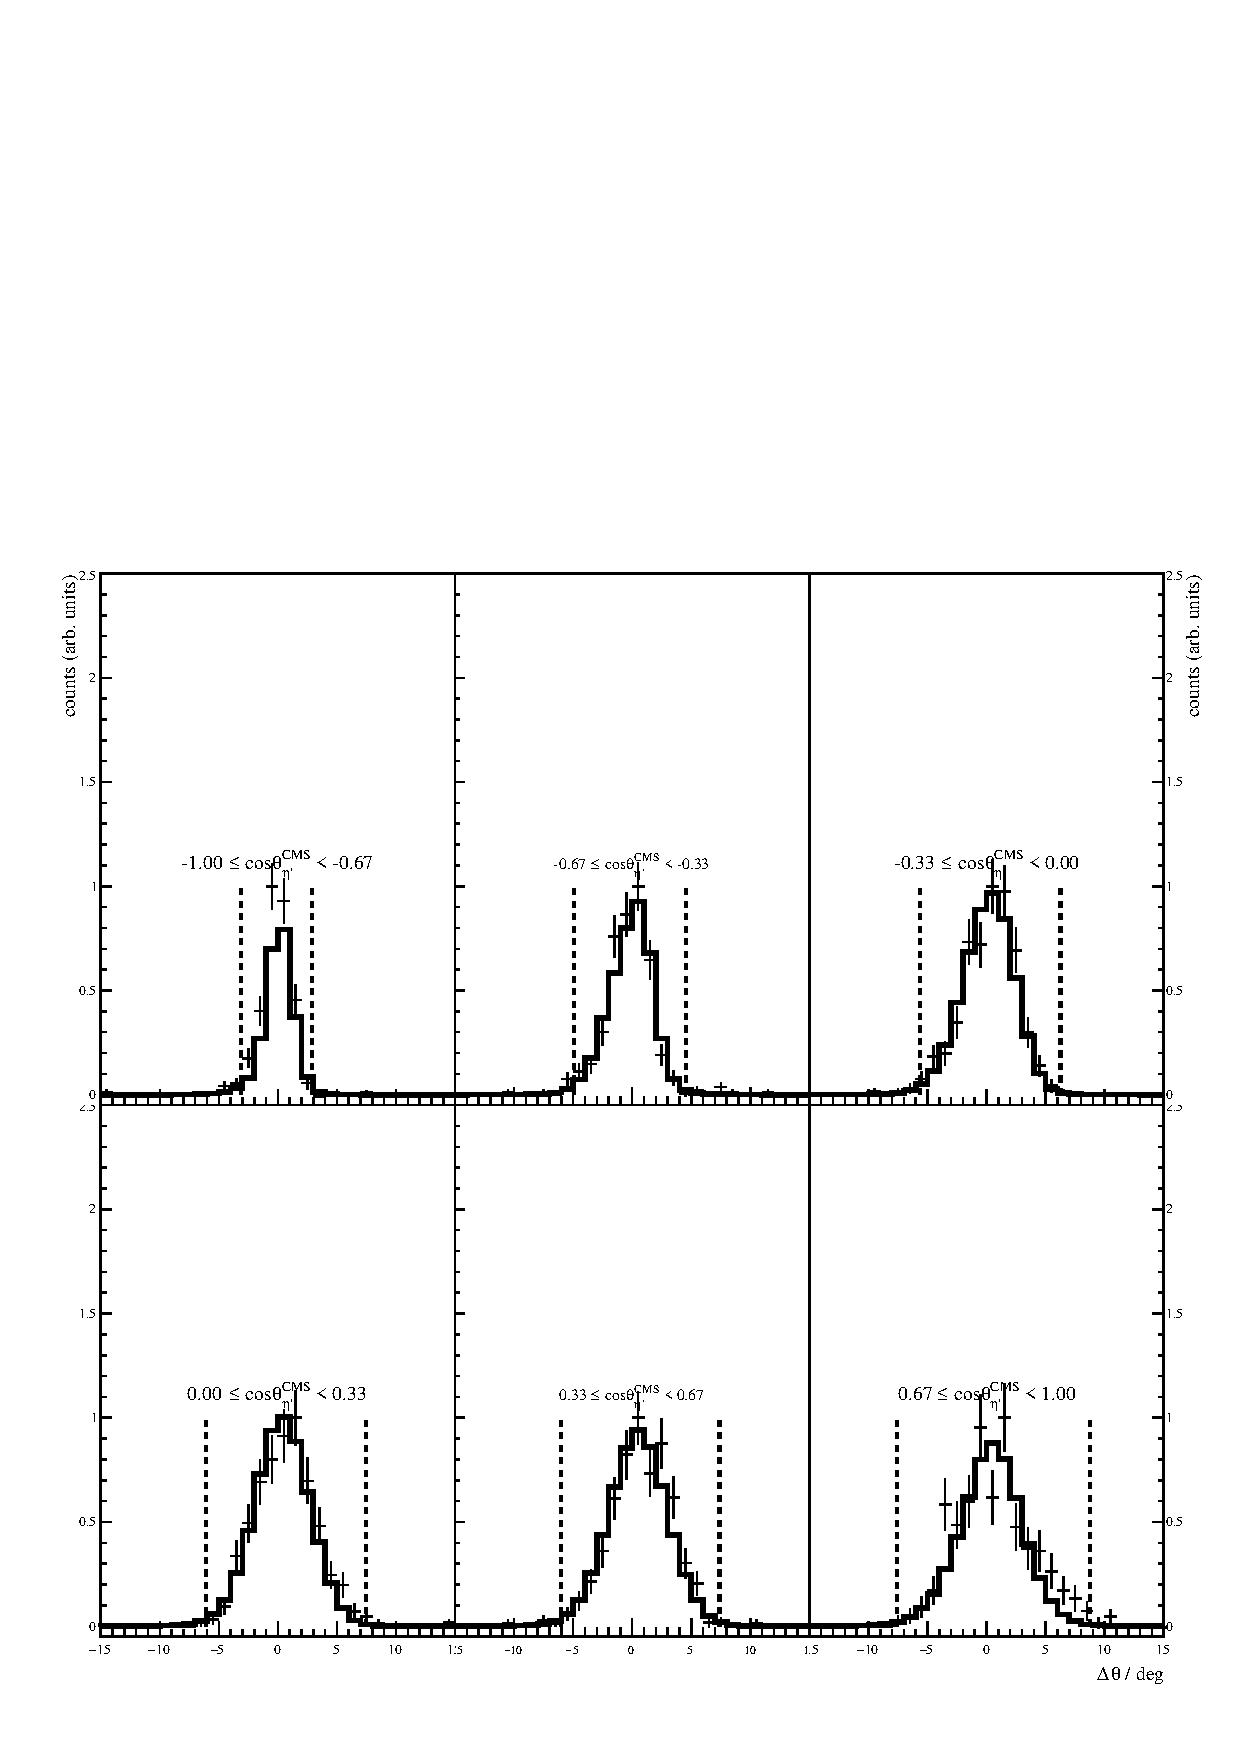
\includegraphics[width=\linewidth]{../figs/hydrogen/bin_cuts/thetacut_ebin1.pdf}
 	\caption{Polar angle difference of the $p\eta'$ final state with all other cuts applied for the energy bin $\SI{1500}{\mega\eV}\leq E_\gamma<\SI{1600}{\mega\eV}$. The vertical dashed lines show the cut ranges obtained from a gaussian fit to the data (open circles). The solid black histograms represent fitted MC data of $\eta'\to\gamma\gamma$}
 	\label{fig:pol}
 \end{figure}
 \subsubsection{Missing mass}
 The missing mass spectra allow a first investigation of possible background reactions that pass the event selection. For all angular bins of the first energy bin the missing mass is shown in figure \ref{fig:mism}; again, the open circles are the data points with corresponding statistical error bars. The solid colored histograms are fitted MC spectra of different possible background contributions while the black histogram is the signal contribution of $\eta'\to\gamma\gamma$ photoproduction. The turquoise histogram is the sum of all MC histograms. Generally, most of the data can be described by the $\eta'$ MC alone, but especially towards higher masses (and higher beam energies) background contributions extend the missing mass peak as flat background. These are reactions where the reconstructed meson mass $m_\text{meson}^2=E_\text{meson}^2-\vec{p}_\text{meson}^2$ is smaller than the $\eta'$ mass, resulting in larger values for the missing mass. Judging from the fit to the missing mass, $2\pi^0$ and/or $\pi^0\eta$ photoproduction may describe the background as both show similar shapes. All other previously mentioned reactions (table \ref{tab:mc}) do not contribute significantly. However because the spectrum consists only of a narrow peak and the background is flat, fitting the missing mass spectra does not provide many good reference points for the fit to differentiate between contributing reactions. Few events per bin further complicate this. Better conclusions can be drawn from the invariant mass spectra as is discussed in the following. In particular, fitting the invariant mass spectra may reveal background contributions where the fit of missing mass fails to find any, as is the case for the bins in backward direction. The cut ranges for the missing mass are obtained from a \textsc{Novosibirsk} \cite{nov} fit to the data since the missing mass distribution is slightly asymmetric. However, since the tail parameter is small, still a symmetric cut of $\pm2\sigma$ was chosen. It was chosen narrower than the angular cuts to retain less events from 
 background reactions.
  \begin{figure}[htbp]
 	\centering
 	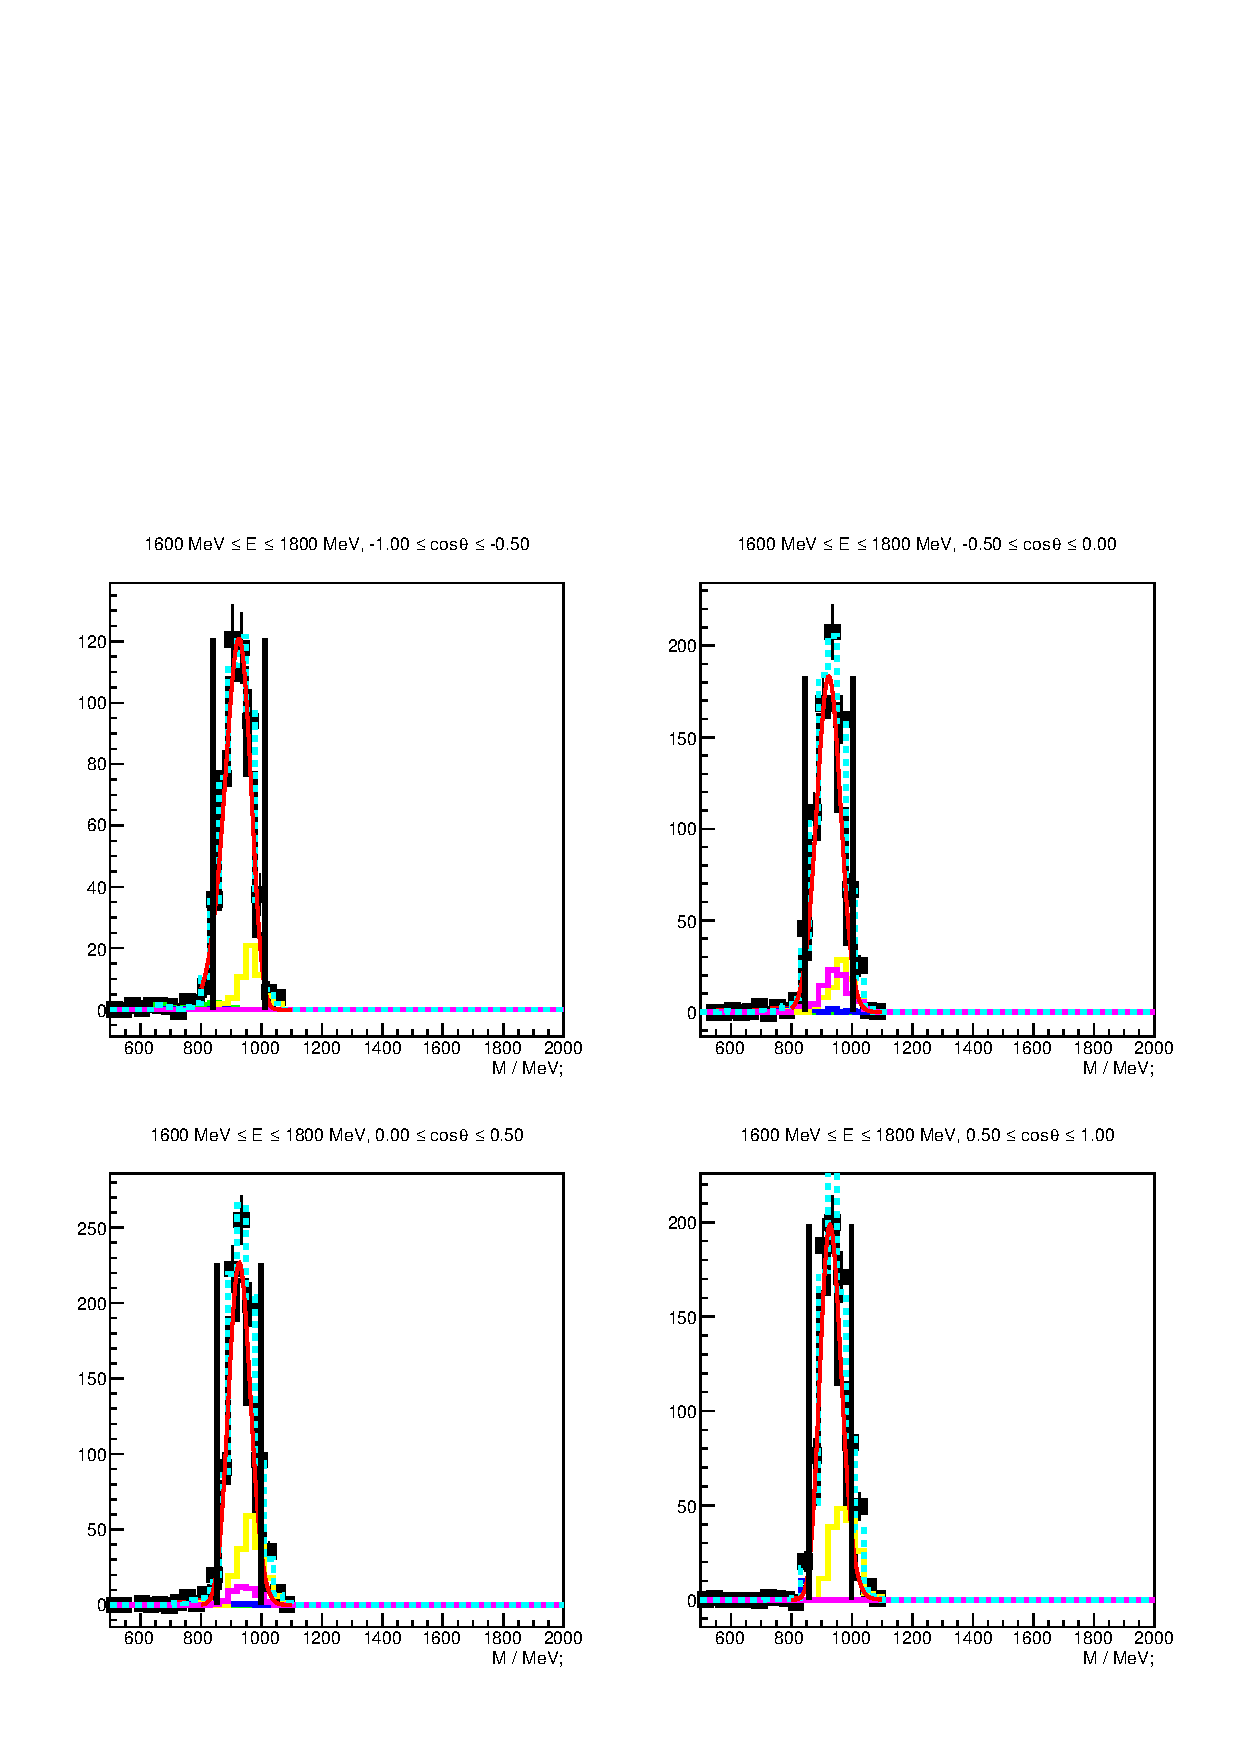
\includegraphics[width=\linewidth]{../figs/hydrogen/bin_cuts/mismcut_ebin1.pdf}
 	\caption{Missing mass of the $p\eta'$ final state with all other cuts applied for the energy bin $\SI{1500}{\mega\eV}\leq E_\gamma<\SI{1600}{\mega\eV}$. The vertical dashed lines show the cut ranges obtained from a fit to data (open circles) employing a \textsc{Novosibirsk} function. The solid colored histograms represent fitted MC data from relevant  photoproduction reactions: in black $\eta'$, in green $\pi^0$, in red $\eta$, in blue $\omega$, in yellow $2\pi^0$, magenta $\pi^0\eta$. The turquoise histogram is the sum of all MC histograms.}
 	\label{fig:mism}
 \end{figure}
 \subsubsection{Invariant mass}
 Investigating the invariant mass spectrum of the final state photons allows to illustrate the impact of the event selection so far. As it has been mentioned all cuts considered up to this point apply to arbitrary meson photoproduction. This means that the invariant mass spectrum will depict peaks belonging to mesons produced in the considered beam energy range. This is shown in Figure \ref{fig:globalinv} giving an overview over all energy and angular bins. All other cuts have been applied. The open circles represent data points and the different colored histograms MC data from relevant competing final states while the black histogram shows the signal contribution of $\eta'$ MC. The turquoise histogram is the sum of all MC contributions and describes the data very well. It has again been found that no other than the shown final states contribute significantly or improve the description of data by MC spectra. As expected one can observe peaks belonging to $\pi^0,\eta, \omega$ and $\eta'$ photoproduction. A flat background underneath the complete spectrum is realized by $2\pi^0$ and $\pi^0\eta$ final state photons that have been wrongfully combined to two photons. Remarkably, the $\pi^0,\eta$ and $\omega$ invariant mass distributions also depict long tails towards lower and higher masses, although they contribute only marginally to the sum of all MC spectra (note the logarithmic y-Scale). At least for $\pi^0$ production this can be explained by the fact that one low energetic photon is lost during reconstruction while the (high energetic) proton wrongfully creates two tracks of which one is then combined with the other photon as meson candidate \cite{farahphd}. It is likely similar mechanisms are responsible for the other reactions.
 \begin{figure}[htbp]
	\centering
	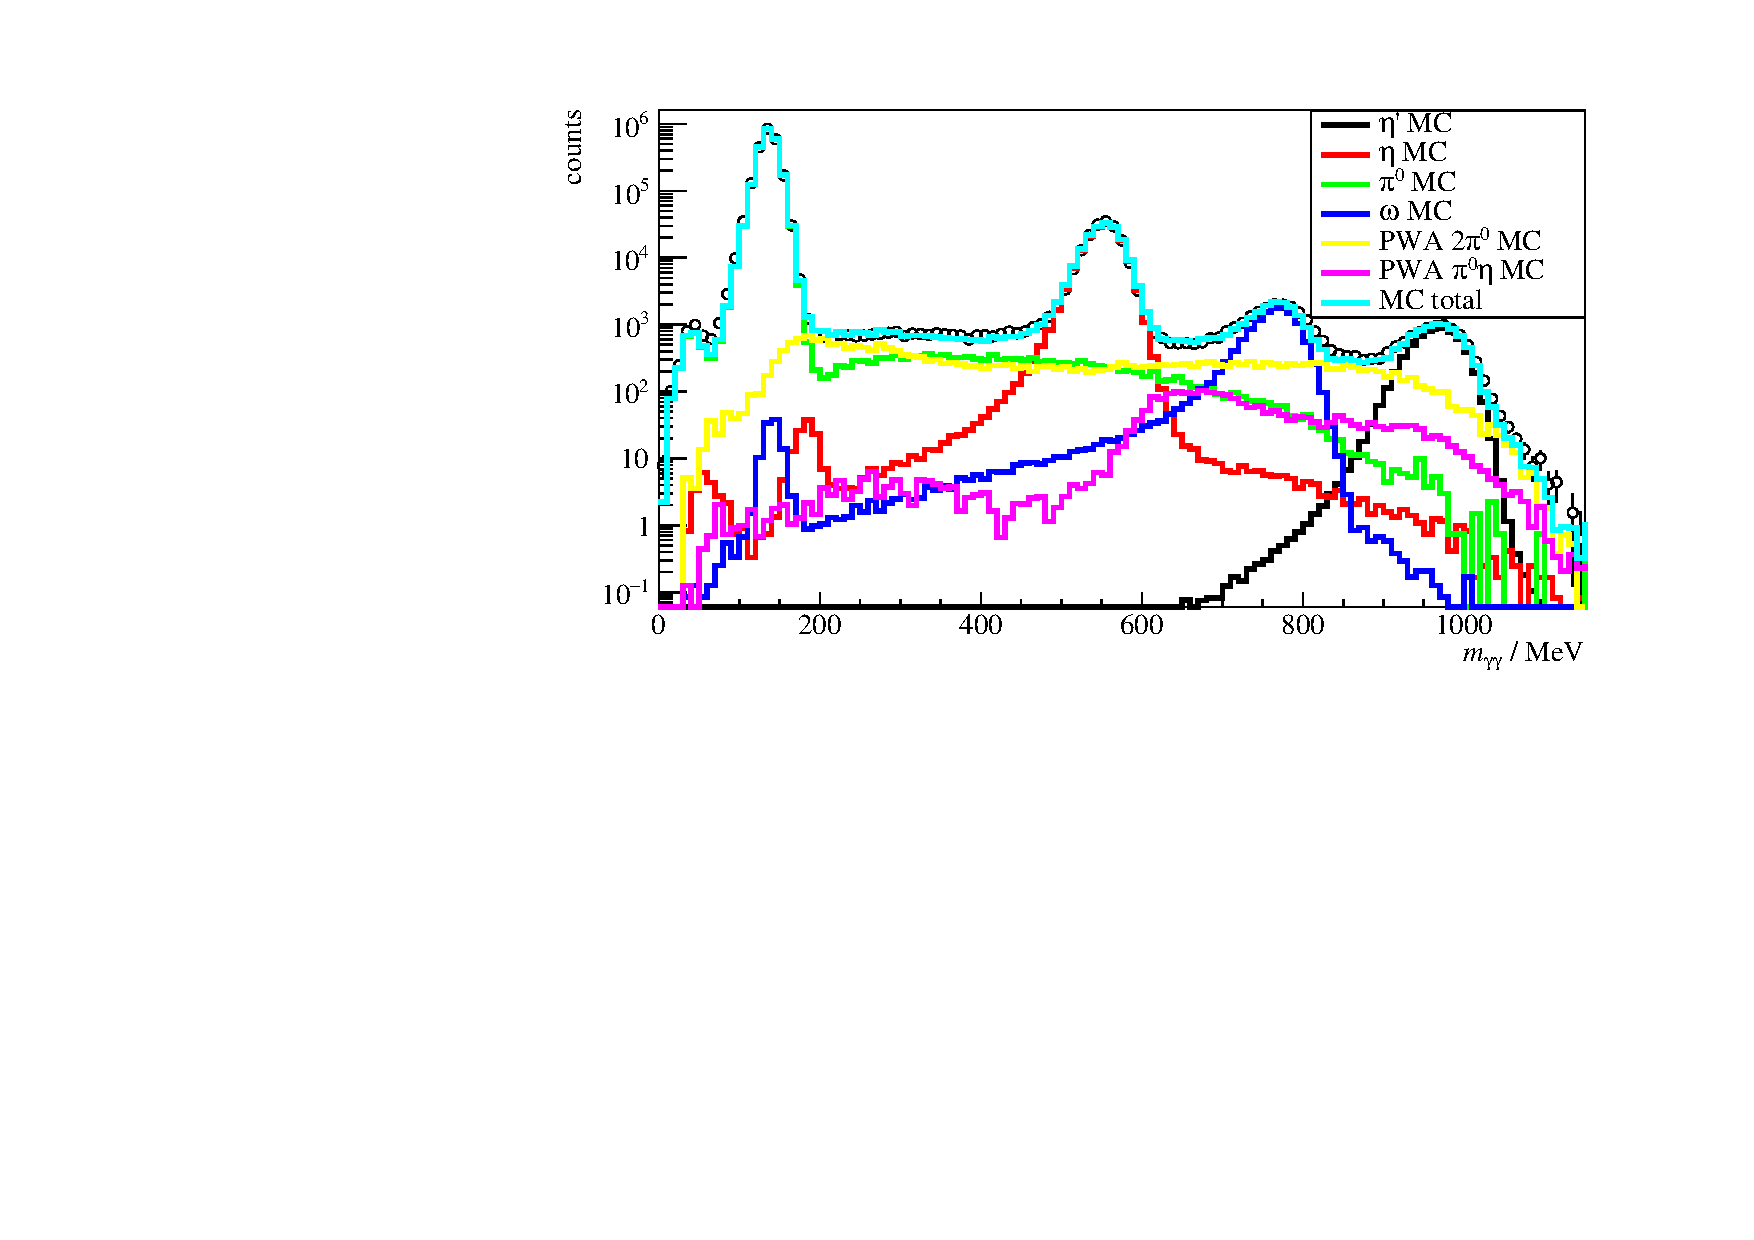
\includegraphics[width=\linewidth]{../figs/hydrogen/invm_global.pdf}
	\caption{Invariant mass of the $p\eta'$ final state with all other cuts applied for all energy and angular bins. The open circles represent the measured data, the solid colored histograms fitted MC data from relevant photoproduction reactions: in black $\eta'$, in green $\pi^0$, in red $\eta$, in blue $\omega$, in yellow $2\pi^0$ and in magenta $\pi^0\eta$. The turquoise histogram is the sum of all MC histograms.}
	\label{fig:globalinv}
\end{figure} 
To finally select only $\eta'$ photoproduction event candidates the invariant mass cut is determined again in bins of beam energy and meson polar angle. This is shown in figure \ref{fig:invm} for the first energy bin with all angular bins. Here, the same color coding as before applies, but the range of the invariant mass has been reduced to only cover the $\eta'$ peak for visibility's sake. Additionally the cut ranges, representing a $2\sigma$ interval obtained from a gaussian fit to the $\eta'$ MC, are shown as dashed, red lines. Considering the statistics the MC spectra still describe the data well. It is found again that the significant background contributions in the invariant mass range of interest are given by $2\pi^0$ and $\pi^0\eta$ photoproduction.  
\begin{figure}[htbp]
 	\centering
 	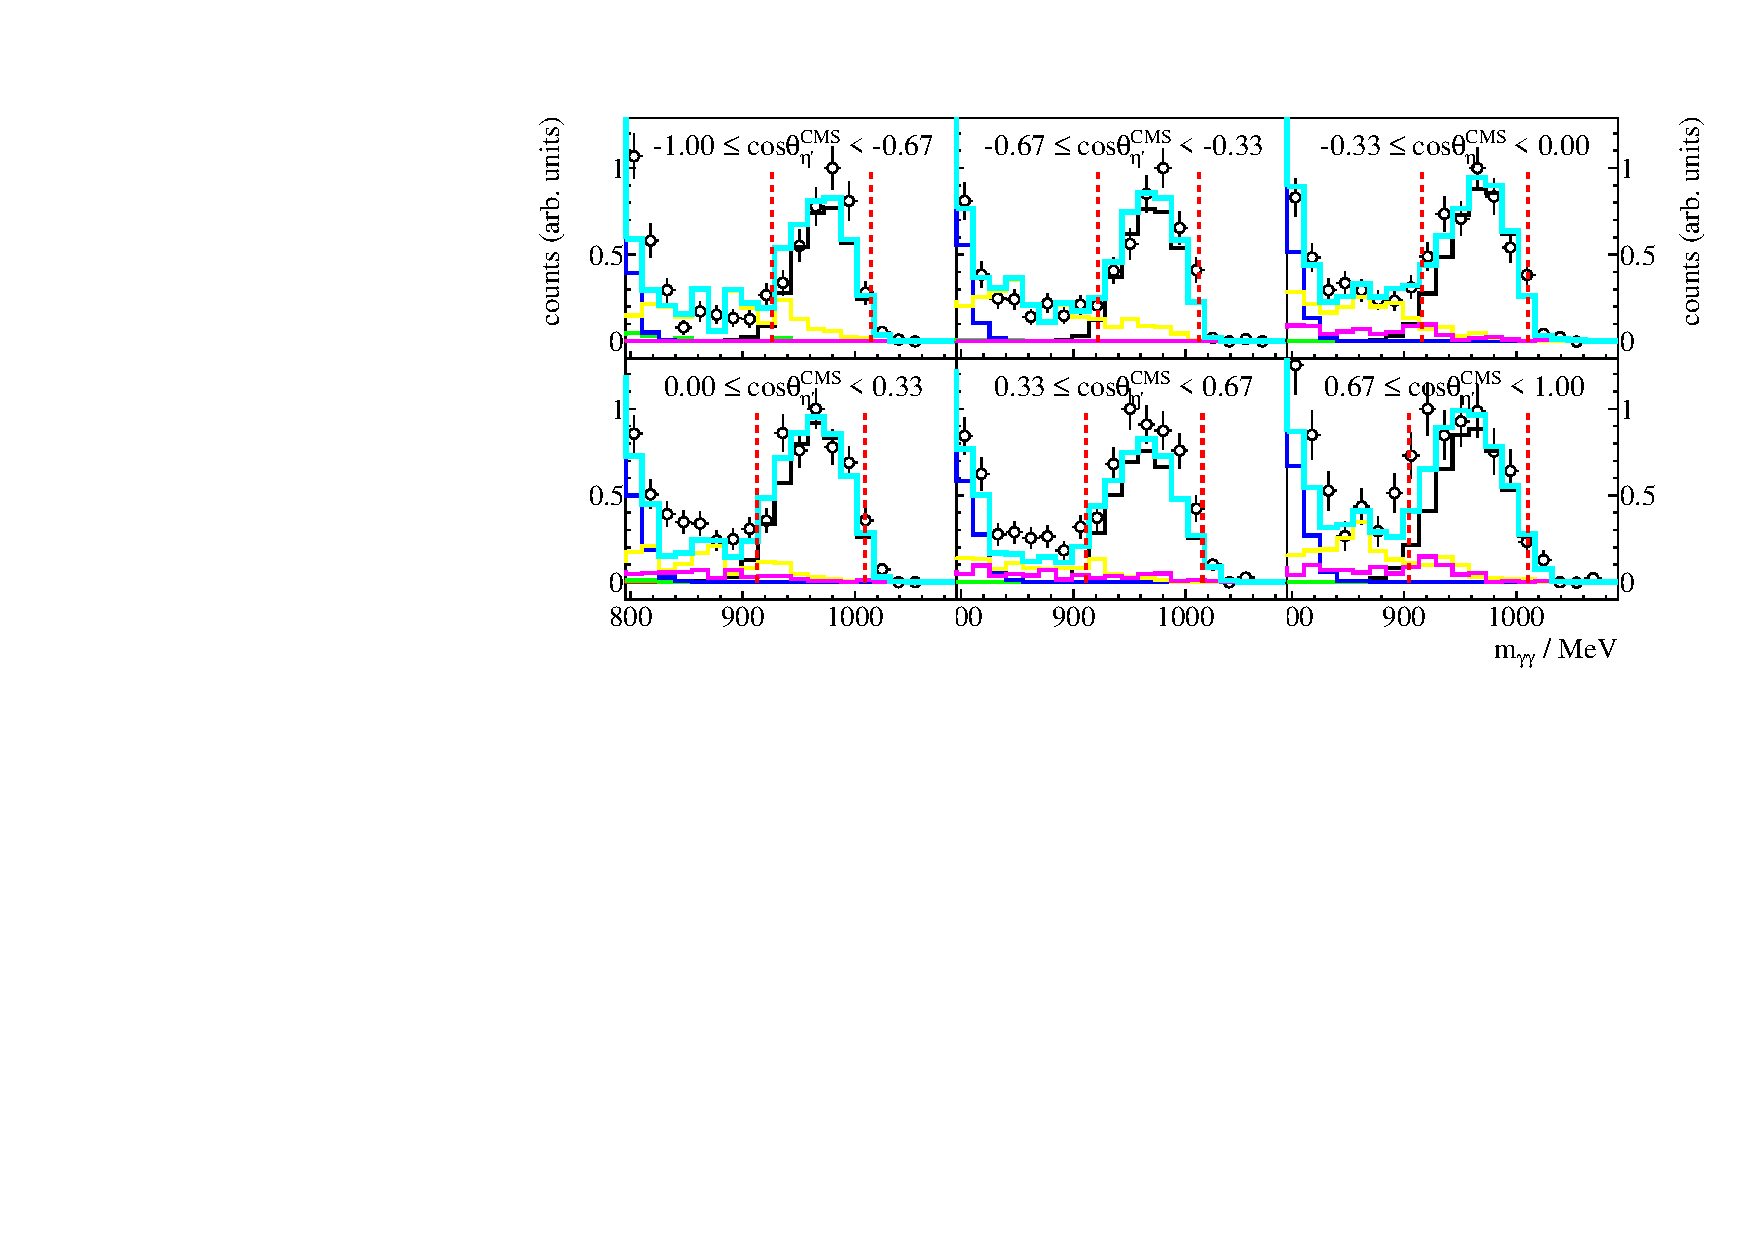
\includegraphics[width=\linewidth]{../figs/hydrogen/bin_cuts/invcut_ebin1.pdf}
 	\caption{Invariant mass of the $p\eta'$ final state with all other cuts applied for the energy bin $\SI{1500}{\mega\eV}\leq E_\gamma<\SI{1600}{\mega\eV}$. The vertical dashed lines show the cut ranges obtained from a gaussian fit to the $\eta'$ MC data (solid black histogram). The open circles represent the measured data, the solid colored histograms fitted MC data from relevant photoproduction reactions: in black $\eta'$, in green $\pi^0$, in red $\eta$, in blue $\omega$, in yellow $2\pi^0$ and in magenta $\pi^0\eta$. The turquoise histogram is the sum of all MC histograms.}
 	\label{fig:invm}
\end{figure}
\subsection{Quality of event selection}
In order to investigate the impact of the applied cuts the detector and analysis acceptance $A(E_\gamma,\cos\theta)$ can be investigated. It is defined as the ratio of reconstructed events $N^\text{rec}(E_\gamma,\cos\theta)$ to generated events $N^\text{gen}(E_\gamma,\cos\theta)$ \begin{equation}
	A:=\frac{N^\text{rec}(E_\gamma,\cos\theta)}{N^\text{gen}(E_\gamma,\cos\theta)}
\end{equation}
and is shown in figure \ref{fig:acc}. Acceptance holes are visible in very forward and in backward direction which can be contributed to events where the proton escapes the calorimeters or is absorbed in insensitive material. Also, events close to threshold are unlikely to be reconstructed which can also be explained by low energy protons and/or low energy photons. A maximum acceptance of $\tilde{A}\approx0.61$ is reached which can be understood considering the cuts that have been made; each $3\sigma$ cuts retains $99\%$ of events and each $2\sigma$ cut $95\%$. Assuming detection efficiencies of $90\%$ for the two uncharged photons and $85\%$ for the charged proton (\cite{farahphd,hartmannphd}) it is evident that $0.99^2\cdot0.95^2\cdot0.9^2\cdot0.85\approx0.61$.
\begin{figure}[htbp]
	\centering
	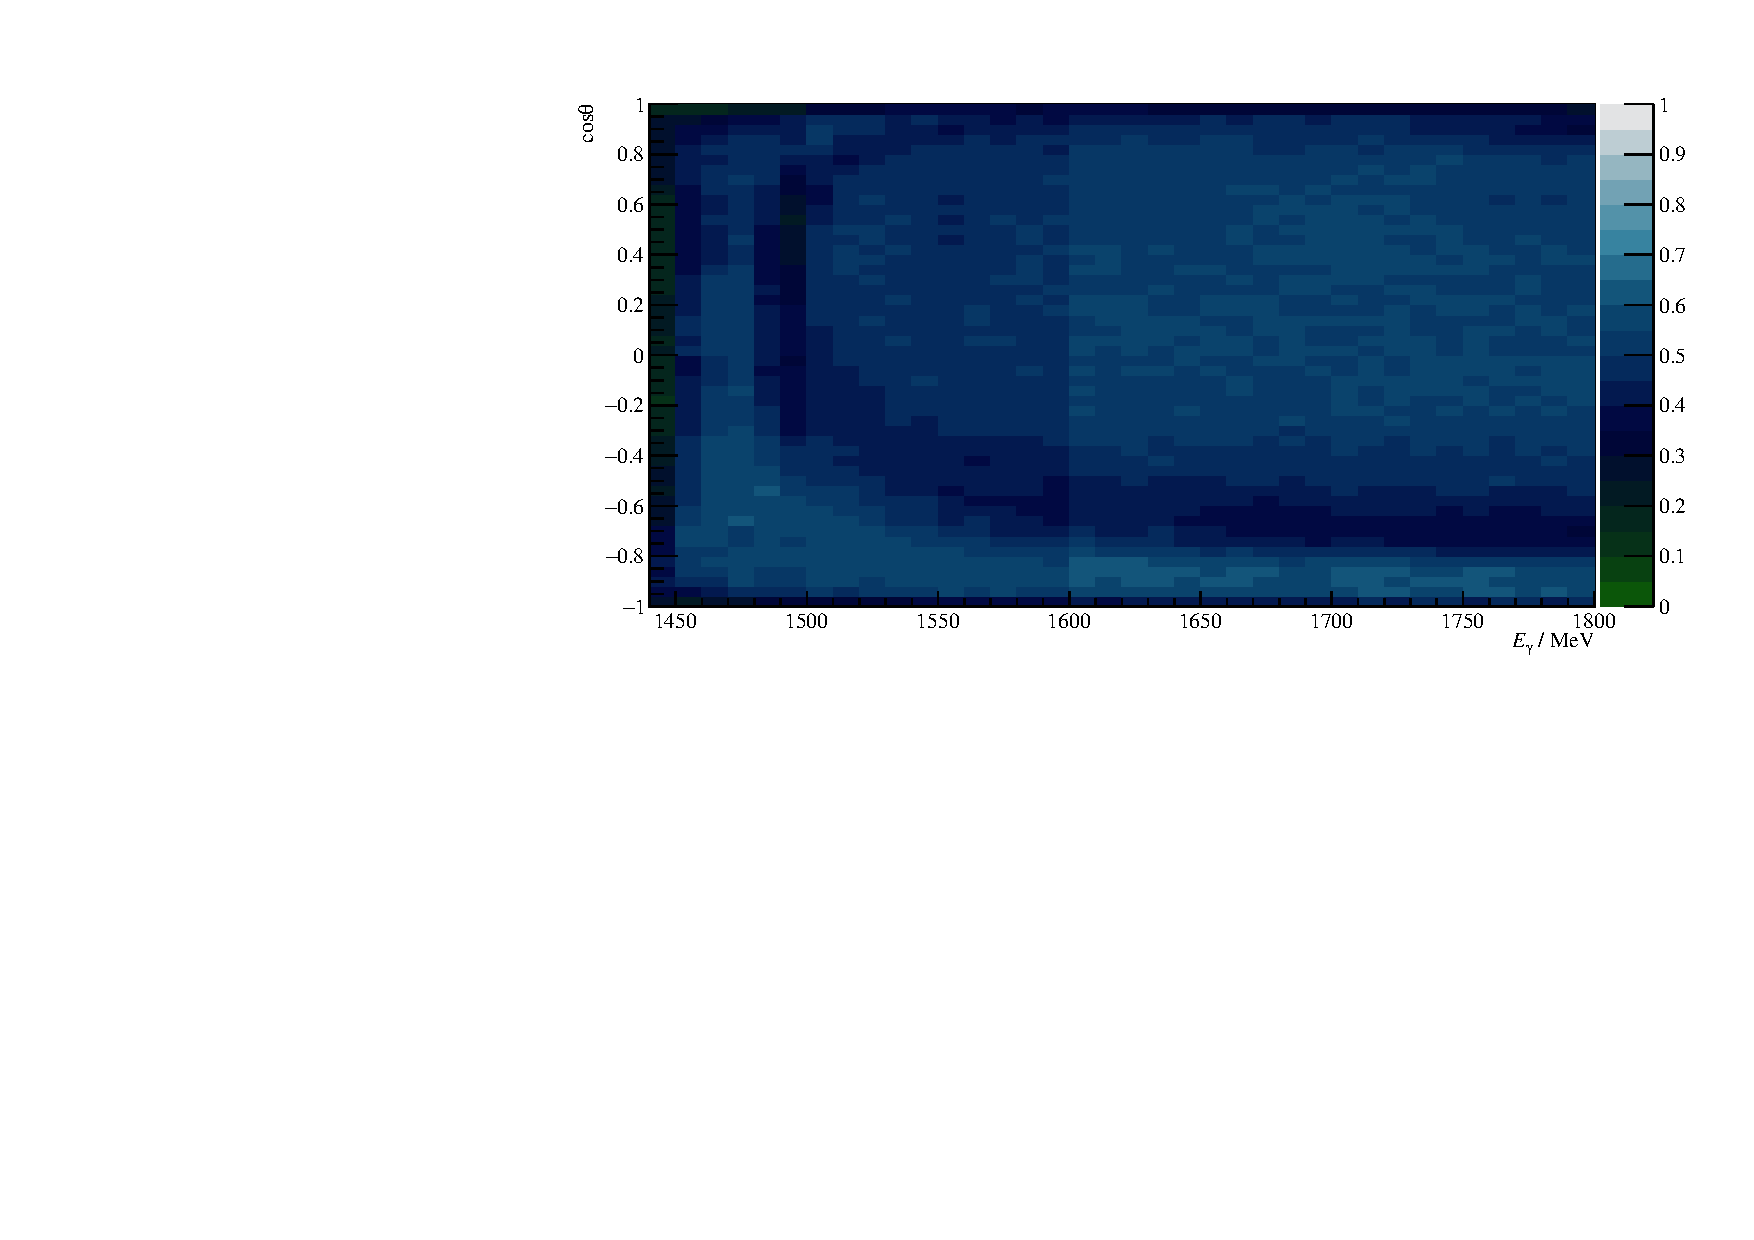
\includegraphics[width=\linewidth]{../figs/hydrogen/acceptance.pdf}
	\caption{Acceptance for the reaction $\gamma p\to p \eta'$ after all cuts that have been discussed so far for 2.5PED and 3PED events}
	\label{fig:acc}
\end{figure}
In total, $8\cdot10^3$ $\eta'$ events were extracted which nonetheless still contain background contaminations. In order to take this into account in the later analysis the fraction of background is determined for each bin in beam energy and meson polar angle. It is estimated as the fraction of total background MC events to total MC events and shown in figure \ref{fig:bkg}. For most bins around $15\%$ of all events are misidentified as $\eta'$ events. Especially at very forward $\cos\theta\to1$ and backward $\cos\theta\to-1$ angles the background contributions are significantly higher, reaching up to $45\%$, which can be traced back to the angular distribution of $\frac{\text{d}\sigma}{\text{d}\Omega}\left(\gamma p \to p\eta'\right)$ \cite{etap_cs}.
\begin{figure}[htbp]
	\centering
	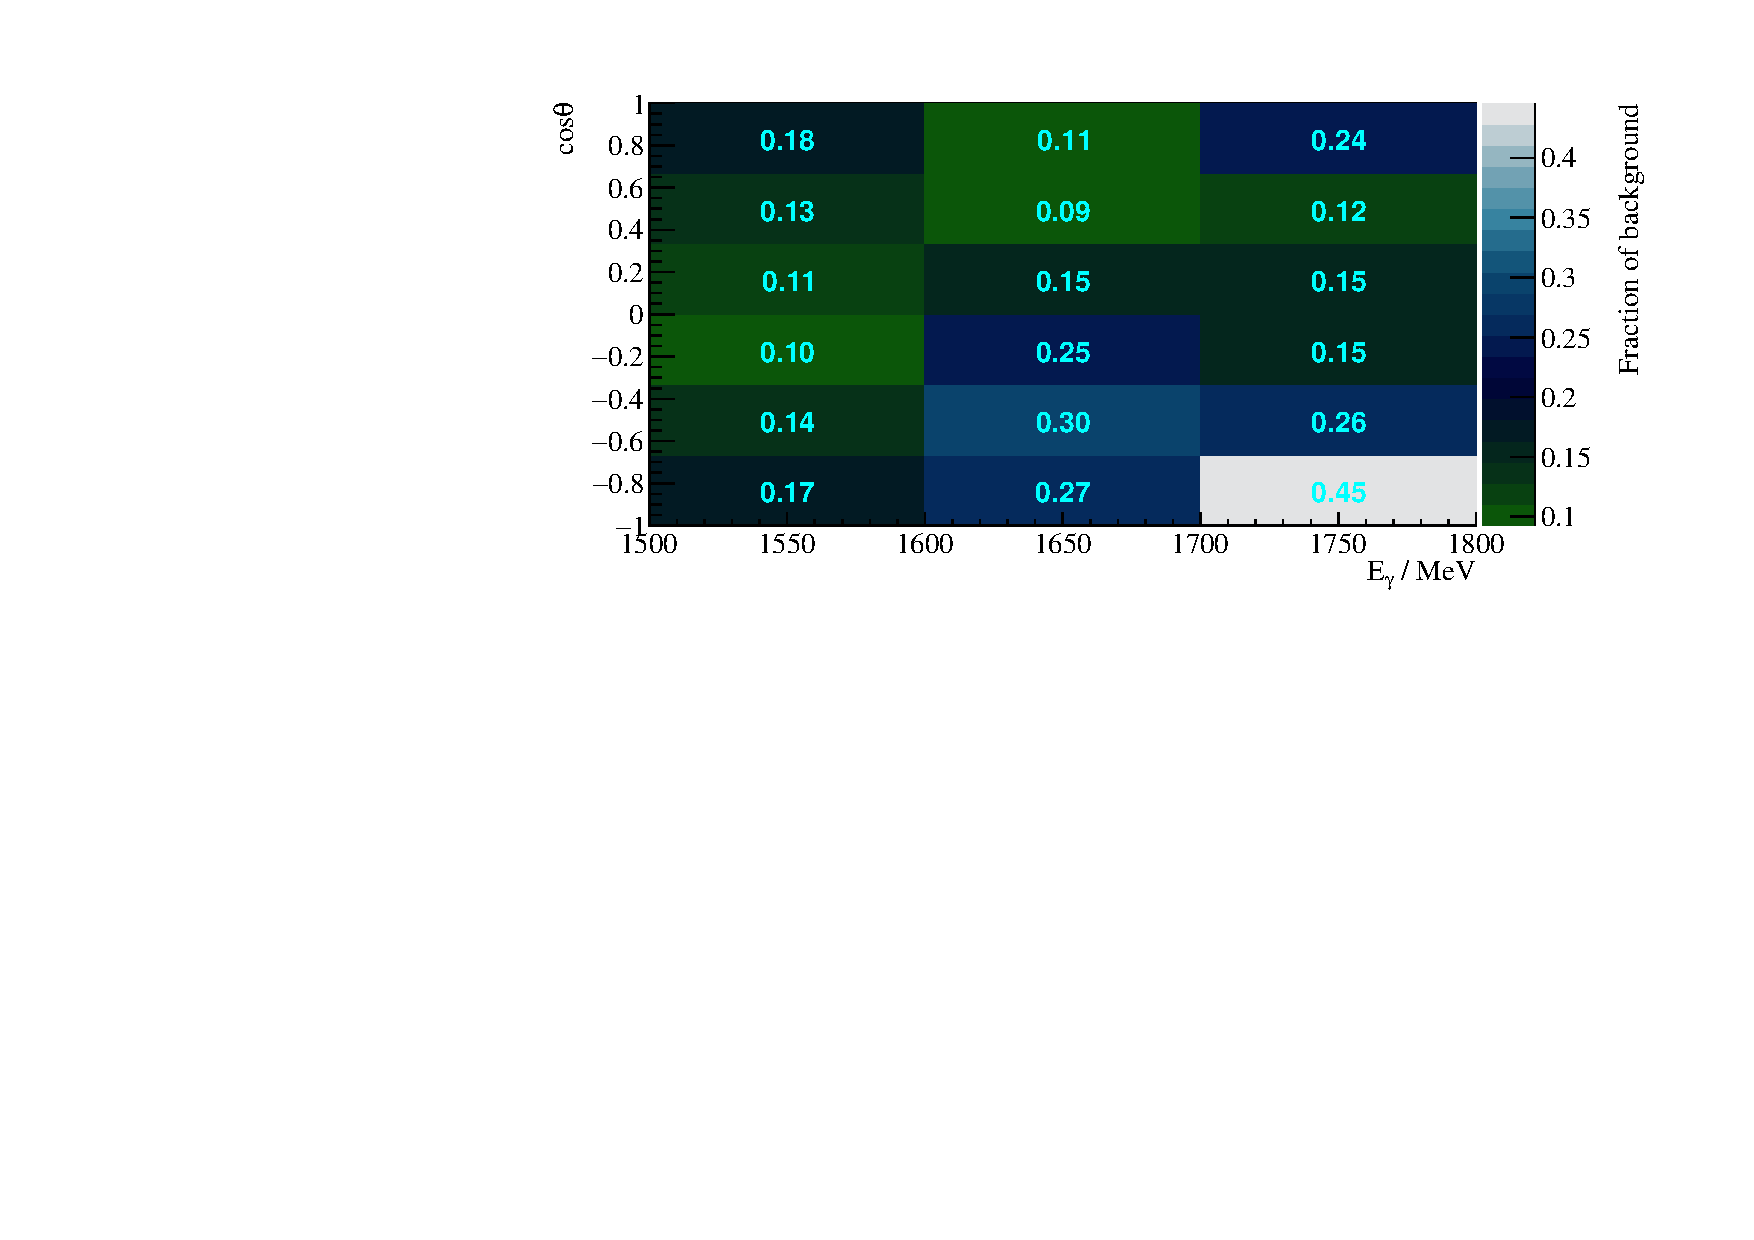
\includegraphics[width=\linewidth]{../figs/hydrogen/bin_cuts/invcut_bkg_percentage.pdf}
	\caption{Fraction of background events in the analyzed beam energy and angular bins.}
	\label{fig:bkg}
\end{figure}

\section{Investigation of background and additional cuts} 
\label{sec:bkg}
So far the background reactions in the $\eta'$ cut ranges have been discussed only phenomenologically as they describe the measured invariant mass spectra best. In the following the plausibility and causality of these background contributions shall be discussed. Furthermore it is investigated if the found background contributions may be reduced or eliminated by additional cut conditions.

\subsection{Inspecting plausibility of background reactions}
To evaluate the likelihood that the background contributions are made up of $2\pi^0$ or $\pi^0\eta$ production events the respective production cross sections in the inspected beam energy region and branching ratios (BR) to purely photonic final states are examined for all considered reactions, see table \ref{tab:plausmc}. Also displayed are the maximum acceptance $\tilde{A}$, which is additionally shown in figure \ref{fig:acc_bkg} for the main background contributions, and the expected background to signal ratio. Since the total number of events is proportional to the cross section $\sigma$, branching ratio BR and acceptance $\tilde{A}$, the ratio of reconstructed background to signal events is then given by 
\begin{equation}
	R=\frac{\sigma\cdot\text{BR}\cdot\tilde{A}}{\sigma_{\eta'}\cdot\text{BR}_{\eta'\to\gamma\gamma}\cdot\tilde{A}_{\eta'}}=\frac{\sigma\cdot\text{BR}\cdot\tilde{A}}{\SI{1}{\micro\barn}\cdot0.022\cdot0.61}.
	\label{eq:r}
\end{equation}
\begin{figure}[htbp]
	\centering
	\begin{subfigure}{\linewidth}
			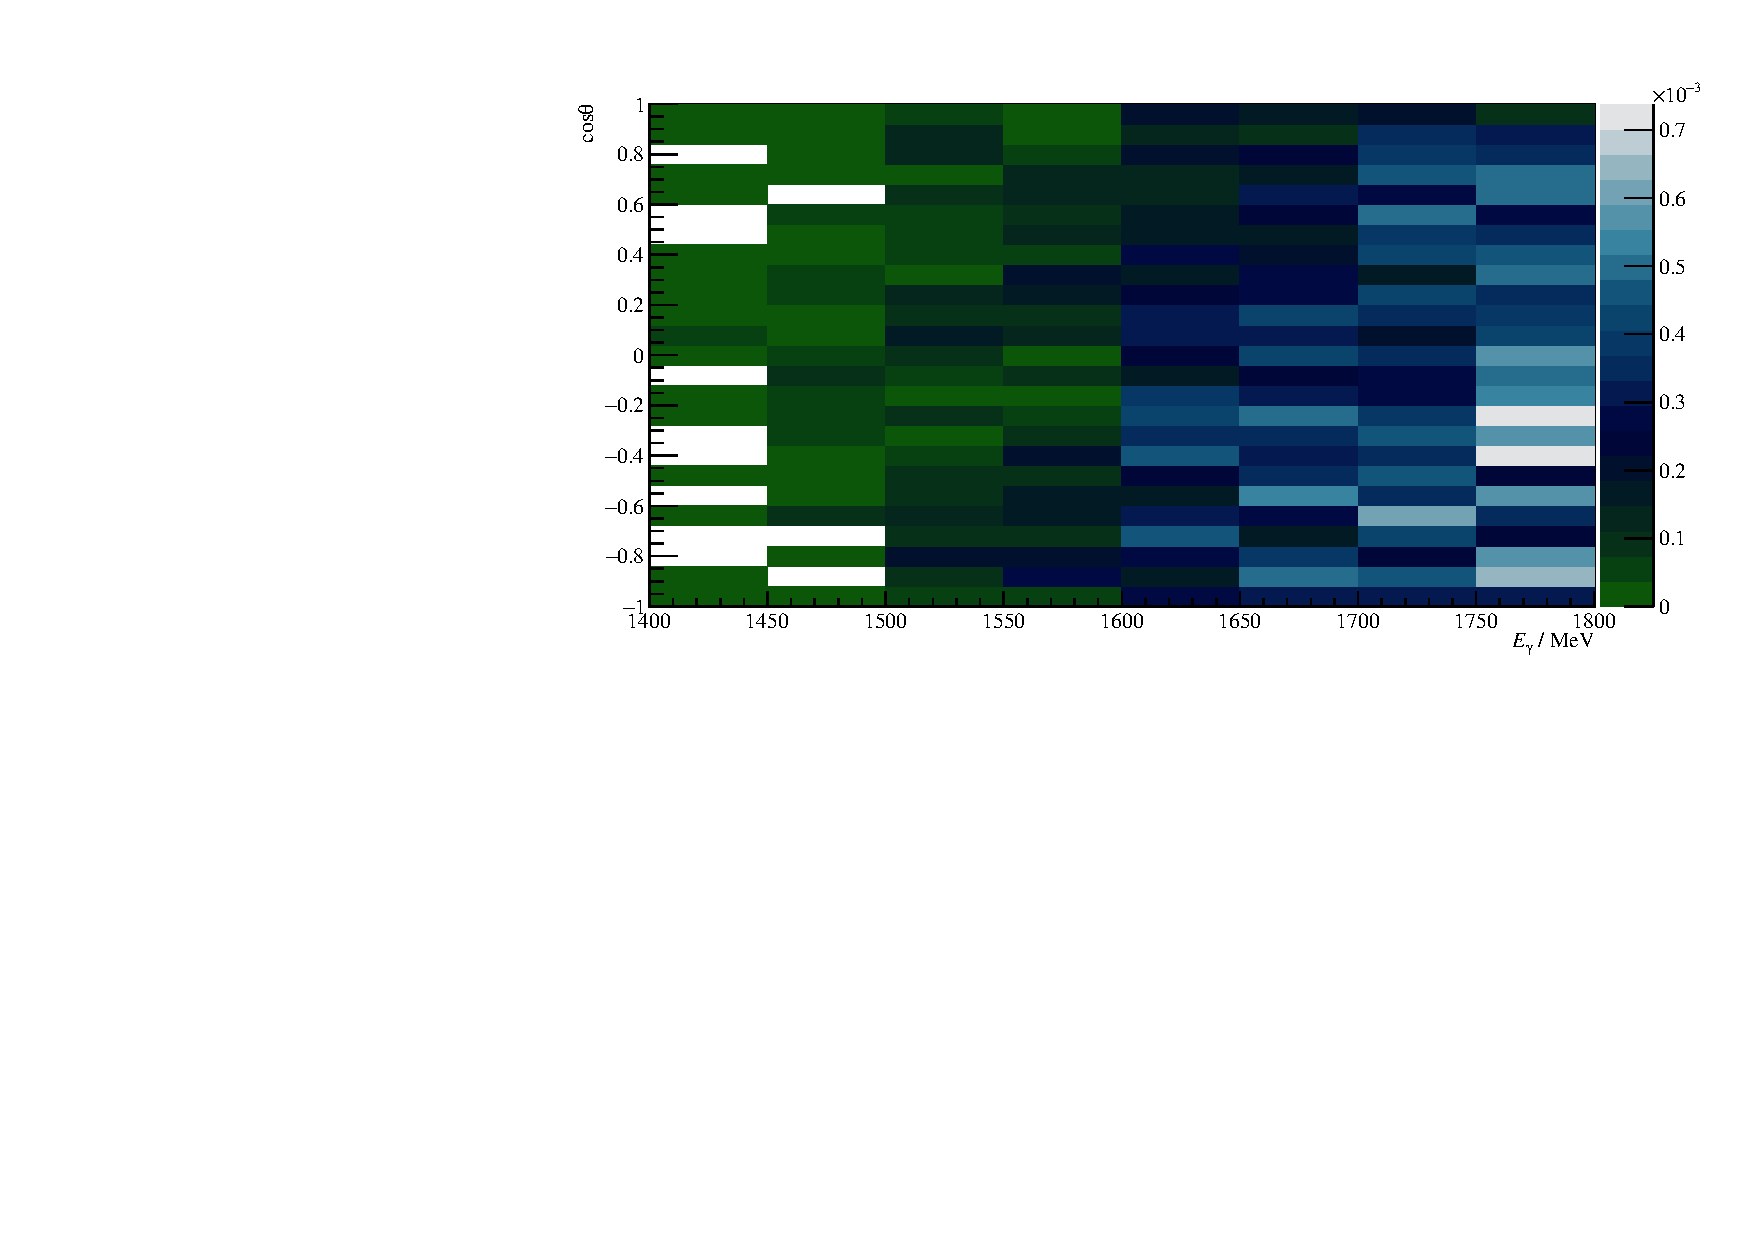
\includegraphics[width=\linewidth]{../figs/hydrogen/acceptance_2pi0.pdf}
			\subcaption{$\gamma p \to p 2\pi^0$}			
	\end{subfigure}
\begin{subfigure}{\linewidth}
		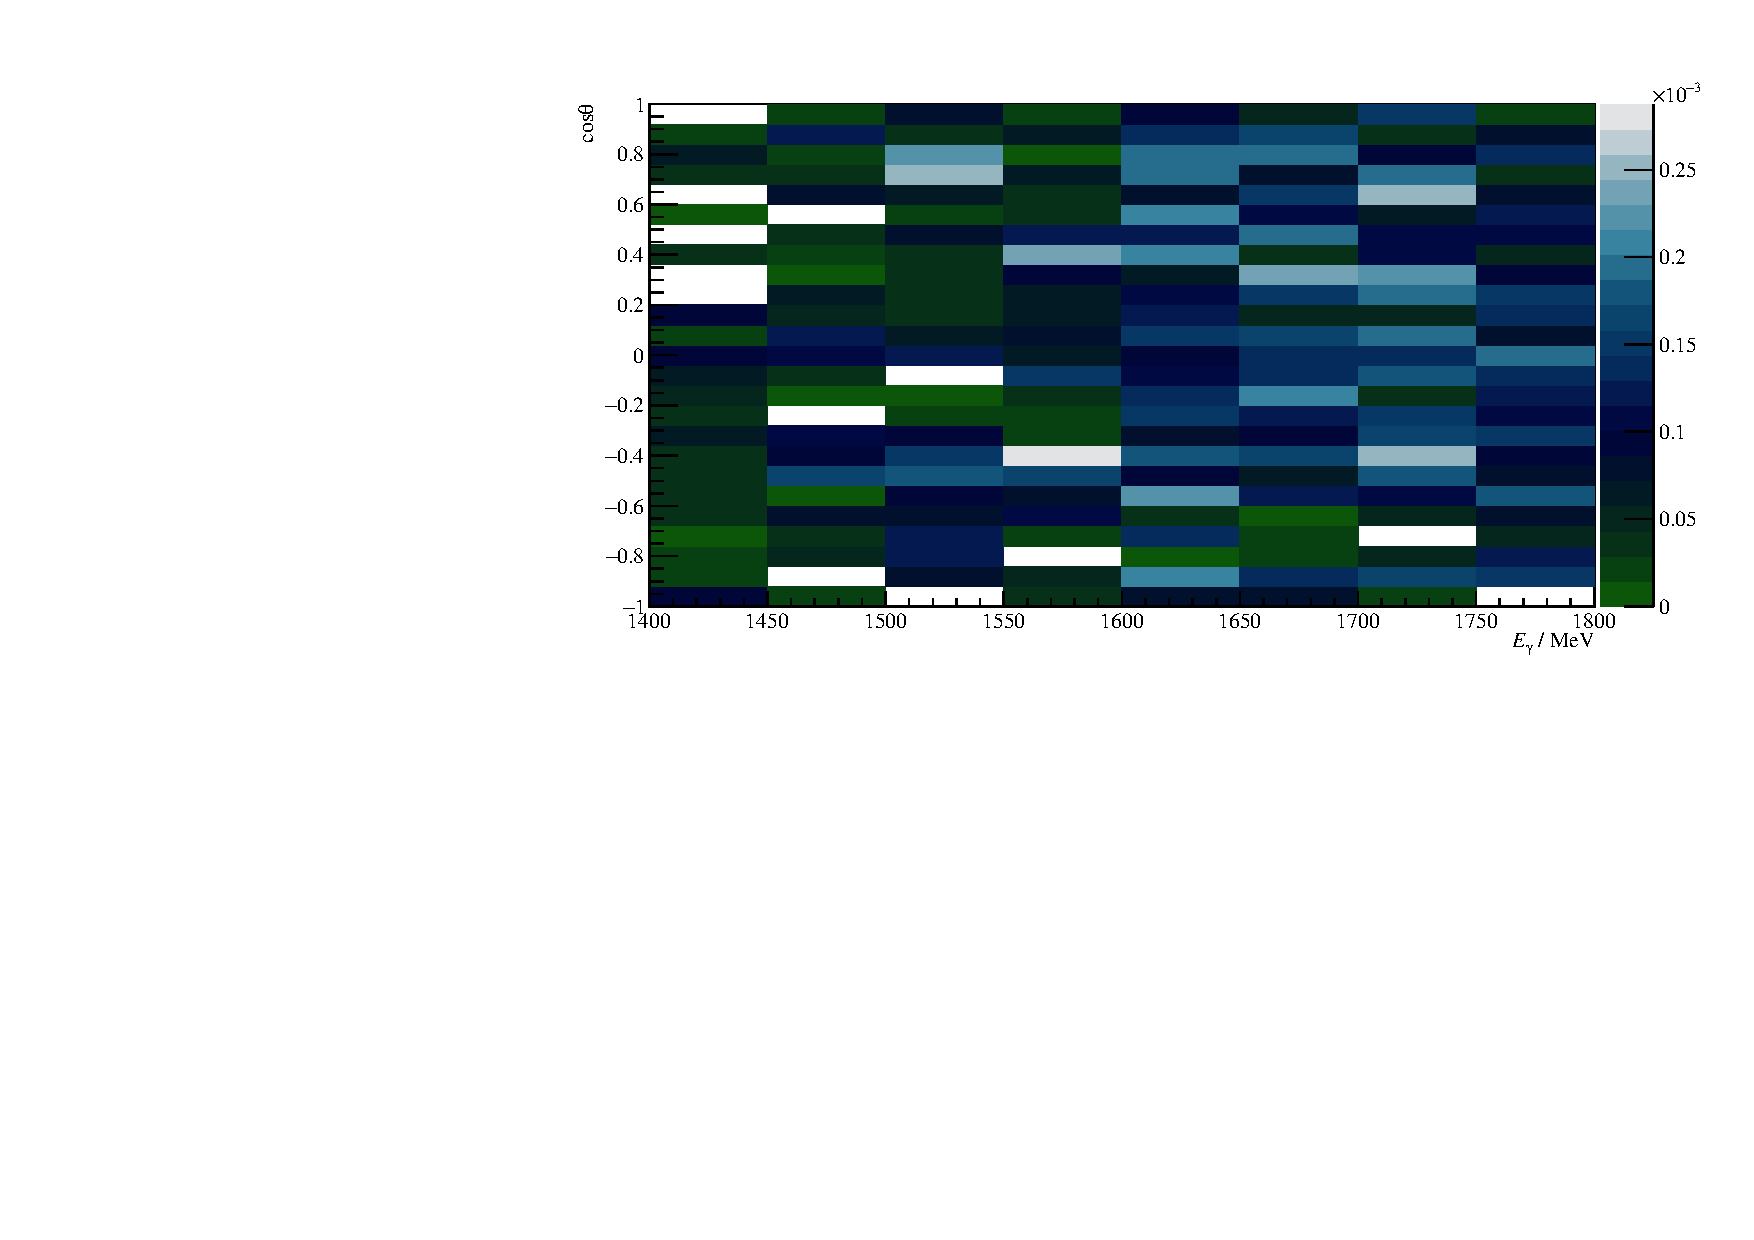
\includegraphics[width=\linewidth]{../figs/hydrogen/acceptance_pi0eta.pdf}
		\subcaption{$\gamma p \to p \pi^0\eta$}
\end{subfigure}
\caption{Acceptance for possible background contributions}
\label{fig:acc_bkg}
\end{figure}

\begin{table}[htbp]
	\centering
	\begin{tabular}{ccccc}
		\toprule
		reaction & $\sigma$ / \si{\micro\barn} & BR\cite{pdg} & $\tilde{A}$&$R$\\
		\hline
		$\gamma p\to p\eta'\to p\gamma\gamma$ &$\approx1$ \cite{etap_cs}& $0.022$ & $0.61$&\\
		$\gamma p\to p2\pi^0\to p4\gamma$ &$\lesssim5$ \cite{2pi0_cs}&$0.9765$& $2\cdot10^{-3}$&0.71\\
		$\gamma p\to p\pi^0\eta\to p 4\gamma$ &$\lesssim3$ \cite{pi0eta_cs} &$0.3948$&$1\cdot 10^{-3}$&0.08\\
		\hline
		$\gamma p \to p\pi^0\to p\gamma\gamma$&$\approx 6$\cite{pi0_cs2}&$0.9882$&$8.3\cdot10^{-7}$&$4\cdot10^{-4}$\\
		$\gamma p \to p\eta\to p\gamma\gamma$&$\approx 2$ \cite{etap_cs}&$0.3996$&$1\cdot10^{-7}$&$7\cdot10^{-6}$\\
		$\gamma p \to p3\pi^0\to p6\gamma$&$\gtrsim 3$\cite{3pi0cs} &$0.9650$&0&0\\
		$\gamma p \to p\omega \to p3\gamma$&$\approx 1$ \cite{omegacs}&$0.0825$&$1\cdot10^{-6}$&$7\cdot10^{-6}$\\
		$\gamma p \to p\pi^+\pi^-$&$\approx40$ \cite{pipics}&-&$1.3\cdot 10^{-6}$&$0.003$\\
		$\gamma p \to n\pi^+$&$\approx 4$ \cite{npiplcs}&-&$1.3\cdot10^{-7}$&$3.8\cdot10^{-5}$\\
		\bottomrule 		
	\end{tabular}
\caption{Total cross sections $\sigma$ in the energy range \SIrange{1500}{1800}{\mega\eV}, branching ratios (BR) to $n\gamma$ final states, maximum acceptance $\tilde{A}$ for signal and possible background contributions as well as the expected signal to background ratio $R$. References \cite{2pi0_cs} and \cite{pi0eta_cs} give the cross sections only up to roughly \SI{1500}{\mega\eV}, the given values are thus upper bounds. For the same reason, from reference \cite{3pi0cs} only a lower bound can be estimated. For all other reactions a rough mean over the energy bins of interest is built. If the references provide only differential cross sections a crude integration in each angular bin is performed. In case only very few $\left(\mathcal{O}\left(10^1\right)\right)$ decays pass event selection, the acceptance is built in one global bin only for the respective reactions. This is indicated by the horizontal line.}
\label{tab:plausmc}
\end{table}
\noindent Almost all reactions exceed $\eta'$ photoproduction in cross section and have a higher BR to purely photonic final states. At the same time the acceptance is almost vanishing, proving that the kinematic cuts are generally very effective. However, despite vanishing acceptance, significant background ratios are expected for $2\pi^0$ and $\pi^0\eta$production, based on equation \eqref{eq:r}. All other reactions only contribute marginally after all cuts and their contribution towards the beam asymmetry can be neglected.  

Although less than $0.2\%$ of two meson production reactions are misidentified as $\eta'$ events they make up a notable portion of background in $\eta'$ data, considering the according branching ratios and cross sections showed. Note that only maximum acceptances and approximations for the cross sections have been used for estimating the  ratio of background events to signal events. As the acceptance and cross sections may vary depending on kinematic bin, also the actual amount of background events may yet vary. Especially in backwards direction the acceptance of $\gamma p \to p\eta'$ events decreases due to escaping protons while at the same time the acceptance for $\gamma p \to p\pi^0\pi^0\to p4\gamma$ and $\gamma p \to p \pi^0\eta\to p 4\gamma$ \emph{increases} in this region towards higher beam energies, see Figure \ref{fig:acc_bkg}. 

Nevertheless, the ratios $R$ are useful to determine the order of magnitude of background contributions. Furthermore the maximum determined ratio of  background events $b$ to total events $\left(s+b\right)$ (Figure \ref{fig:bkg}) and the corresponding value for $R$
\begin{align}
\delta=\frac{s}{s+b}=0.45&&\Leftrightarrow&&R=\frac{b}{s}=\frac{\delta}{1-\delta}=0.81
\end{align} are in very good agreement with the estimated expectations from table \ref{tab:plausmc}. This justifies the previous empirical assumption to only include $2\pi^0$ and $\pi^0\eta$ MC as background reactions in the fit to describe the data.
   
\subsection{Misidentification of background reactions}
It has been reasonably established that the main background reactions that escape the $\eta'$ event selection cuts are realized by $2\pi^0$ and $\pi^0\eta$ production. However, it remains to explain why a four-photon final state is misidentified as $\eta'$ event so that background reducing cuts may be found. In order to do so the MC simulations of the respective final states were investigated. One observes, that for those events that passed the $\eta'$ cuts the generated photon energies for two photons often were of order $E_{\gamma} \sim \mathcal{O}(\SI{e1}{\mega\eV})$ and the other two of order $E_{\gamma} \sim \mathcal{O}(\SI{e2}{\mega\eV})$\footnote{To simplify notation, from now on the four final state photons of the reactions $\gamma p \to p2\pi^0\to p4\gamma$ and $\gamma p \to p\pi^0\eta\to p 4\gamma$ are referred to as $\gamma_1\dots\gamma_4$, where the ascending index corresponds to the photon energy in descending order}. The reconstructed energies however only displayed energies of order $E_{\gamma} \sim \mathcal{O}(\SI{e2}{\mega\eV})$.  During the reconstruction of final state four momenta, a minimum energy of $\SI{20}{\mega\eV}$ per cluster is demanded. This threshold is not passed or only closely passed by $\gamma_3$ and $\gamma_4$ in $2\pi^0$ production for $\sim 60\%$ of all generated photons, see figure \ref{fig:mcgammas_a}.\begin{figure}[htbp]
	\centering
	\begin{subfigure}{\linewidth}
		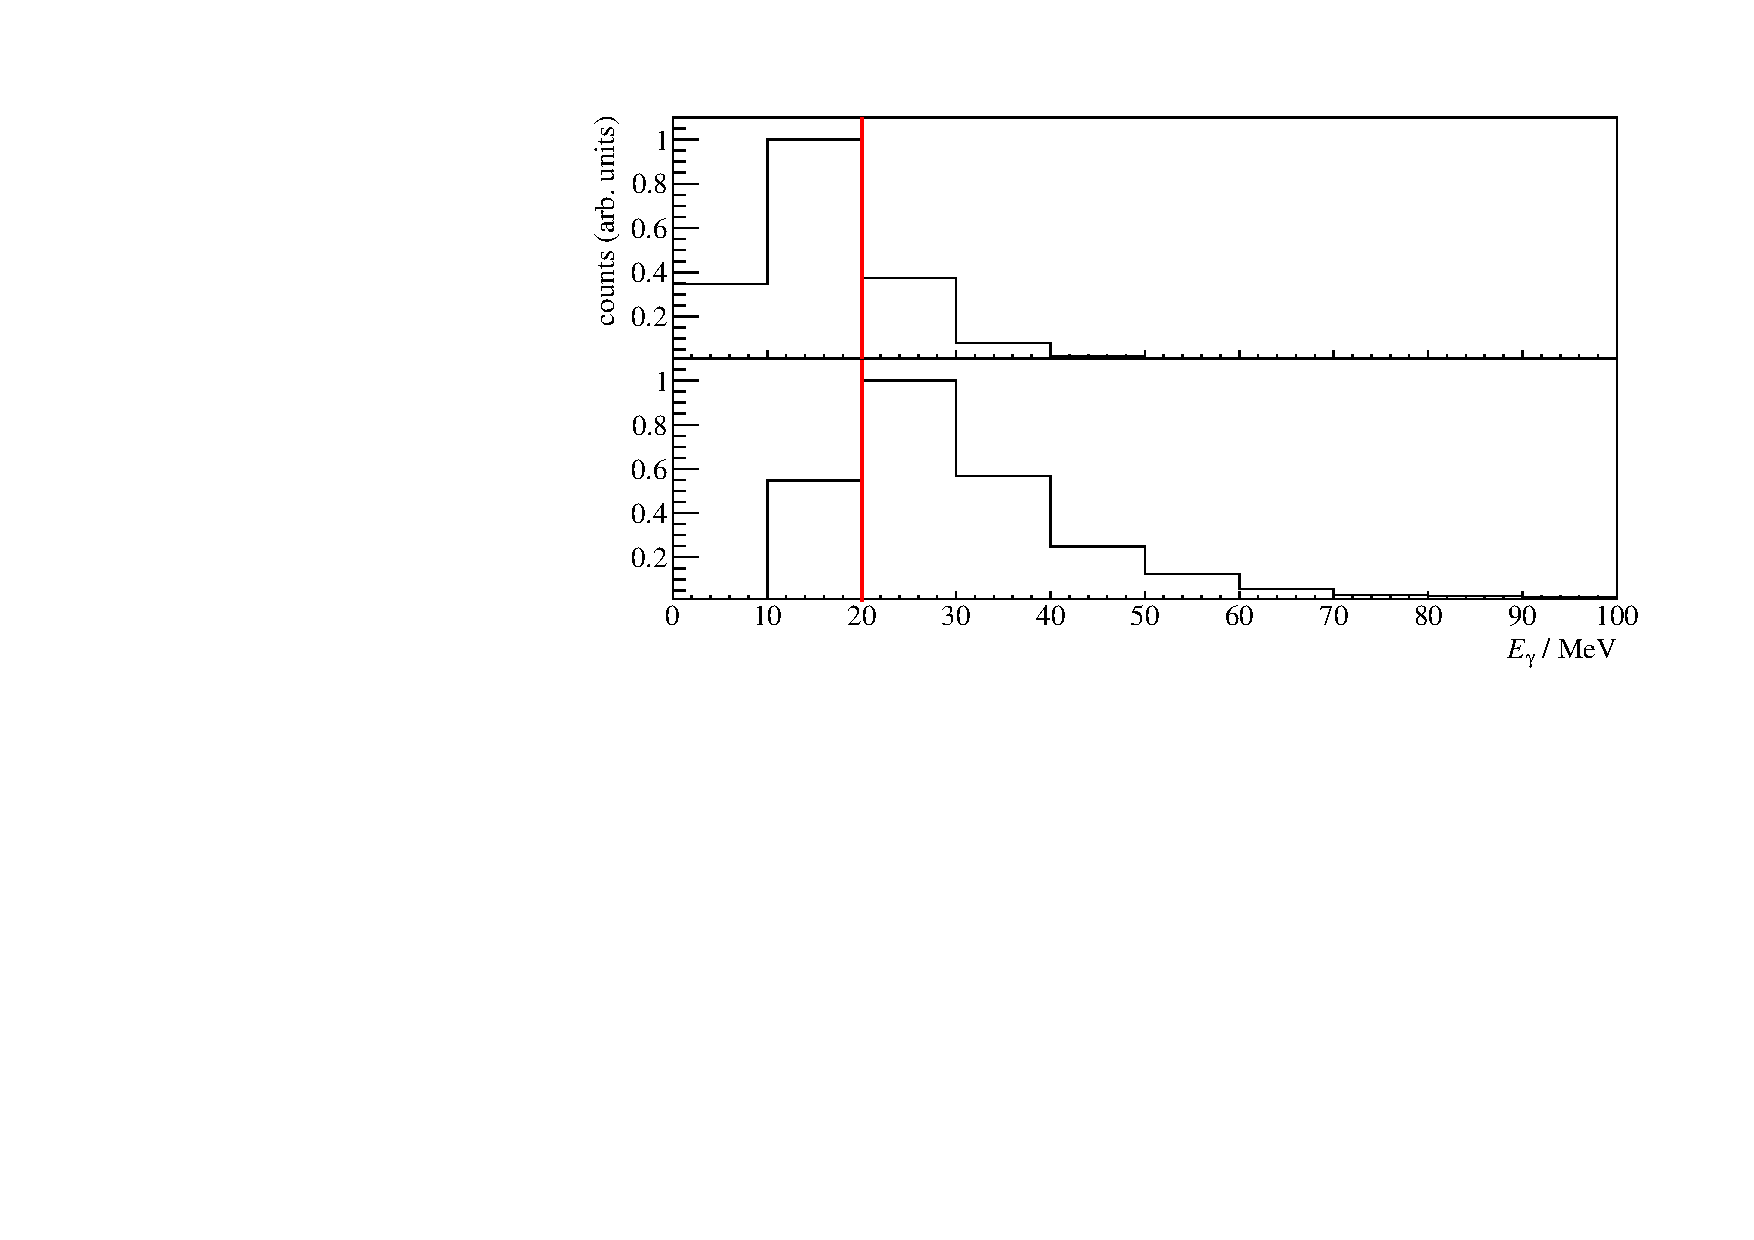
\includegraphics[width=\linewidth]{../figs/hydrogen/mcgammas.pdf}
		\subcaption{Reaction $\gamma p\to p2\pi^0\to 4\gamma$.}
		\label{fig:mcgammas_a}
	\end{subfigure}
	\begin{subfigure}{\linewidth}
		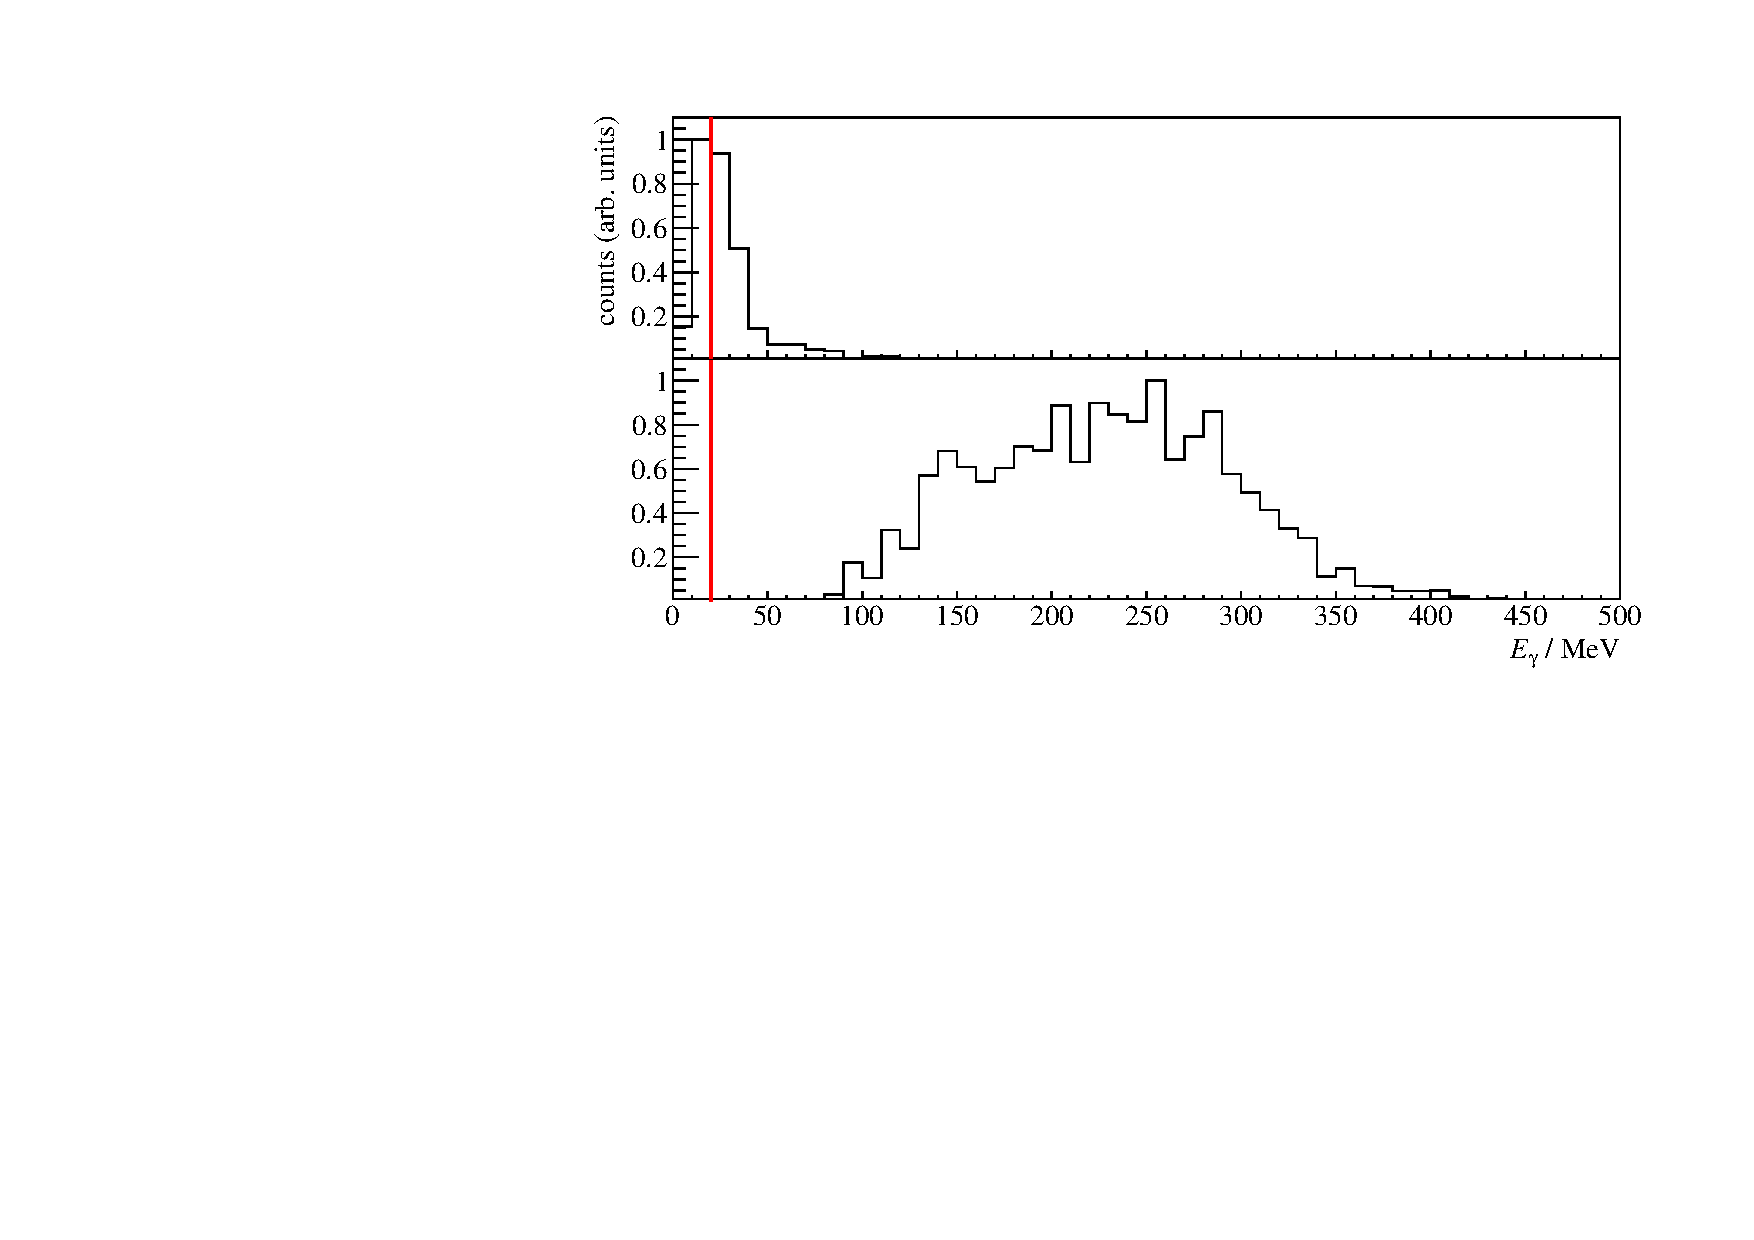
\includegraphics[width=\linewidth]{../figs/hydrogen/mcgammas_pi0eta.pdf}
		\caption{Reaction $\gamma p\to p\pi^0\eta $.}
		\label{fig:mcgammas_b}
	\end{subfigure}			
 				\caption{Generated energies of $\gamma_3$ and $\gamma_4$ in $2\pi^0$ and $\pi^0\eta$ photoproduction MC data. The threshold of $\SI{20}{\mega\eV}$ is marked by a vertical red line. $E_{\gamma_4}$ is shown on the top, $E_{\gamma_3}$ is shown on the bottom of each figure.}
 \end{figure}
 Similarly, $\sim70\%$ of generated $\pi^0\eta$ events have a final state photon which does not or only closely pass the threshold of $\SI{20}{\mega\eV}$. Other than in $2\pi^0$ reactions, this does only apply for $\gamma_4$ while $\gamma_3$ significantly exceeds the threshold of $\SI{20}{\mega\eV}$, see figure \ref{fig:mcgammas_b}. 
 
 At this point it is important to note that the generated energies are in general larger than the reconstructed energies because energy may be deposited in insensitive detector material. Figures \ref{fig:mcgammas_a} and \ref{fig:mcgammas_b} thus do not necessarily resemble a good approximation of how many photons actually are lost because they simply do not pass the energy treshold during reconstruction. To get a better estimate, the generated energies $E_\gamma^\text{gen}$ of $\gamma_1$ and $\gamma_2$ are compared with the reconstructed energies $E_\gamma^\text{rec}$, see Figure \ref{fig:mcgenvsrec}. 
  \begin{figure}[htbp]
	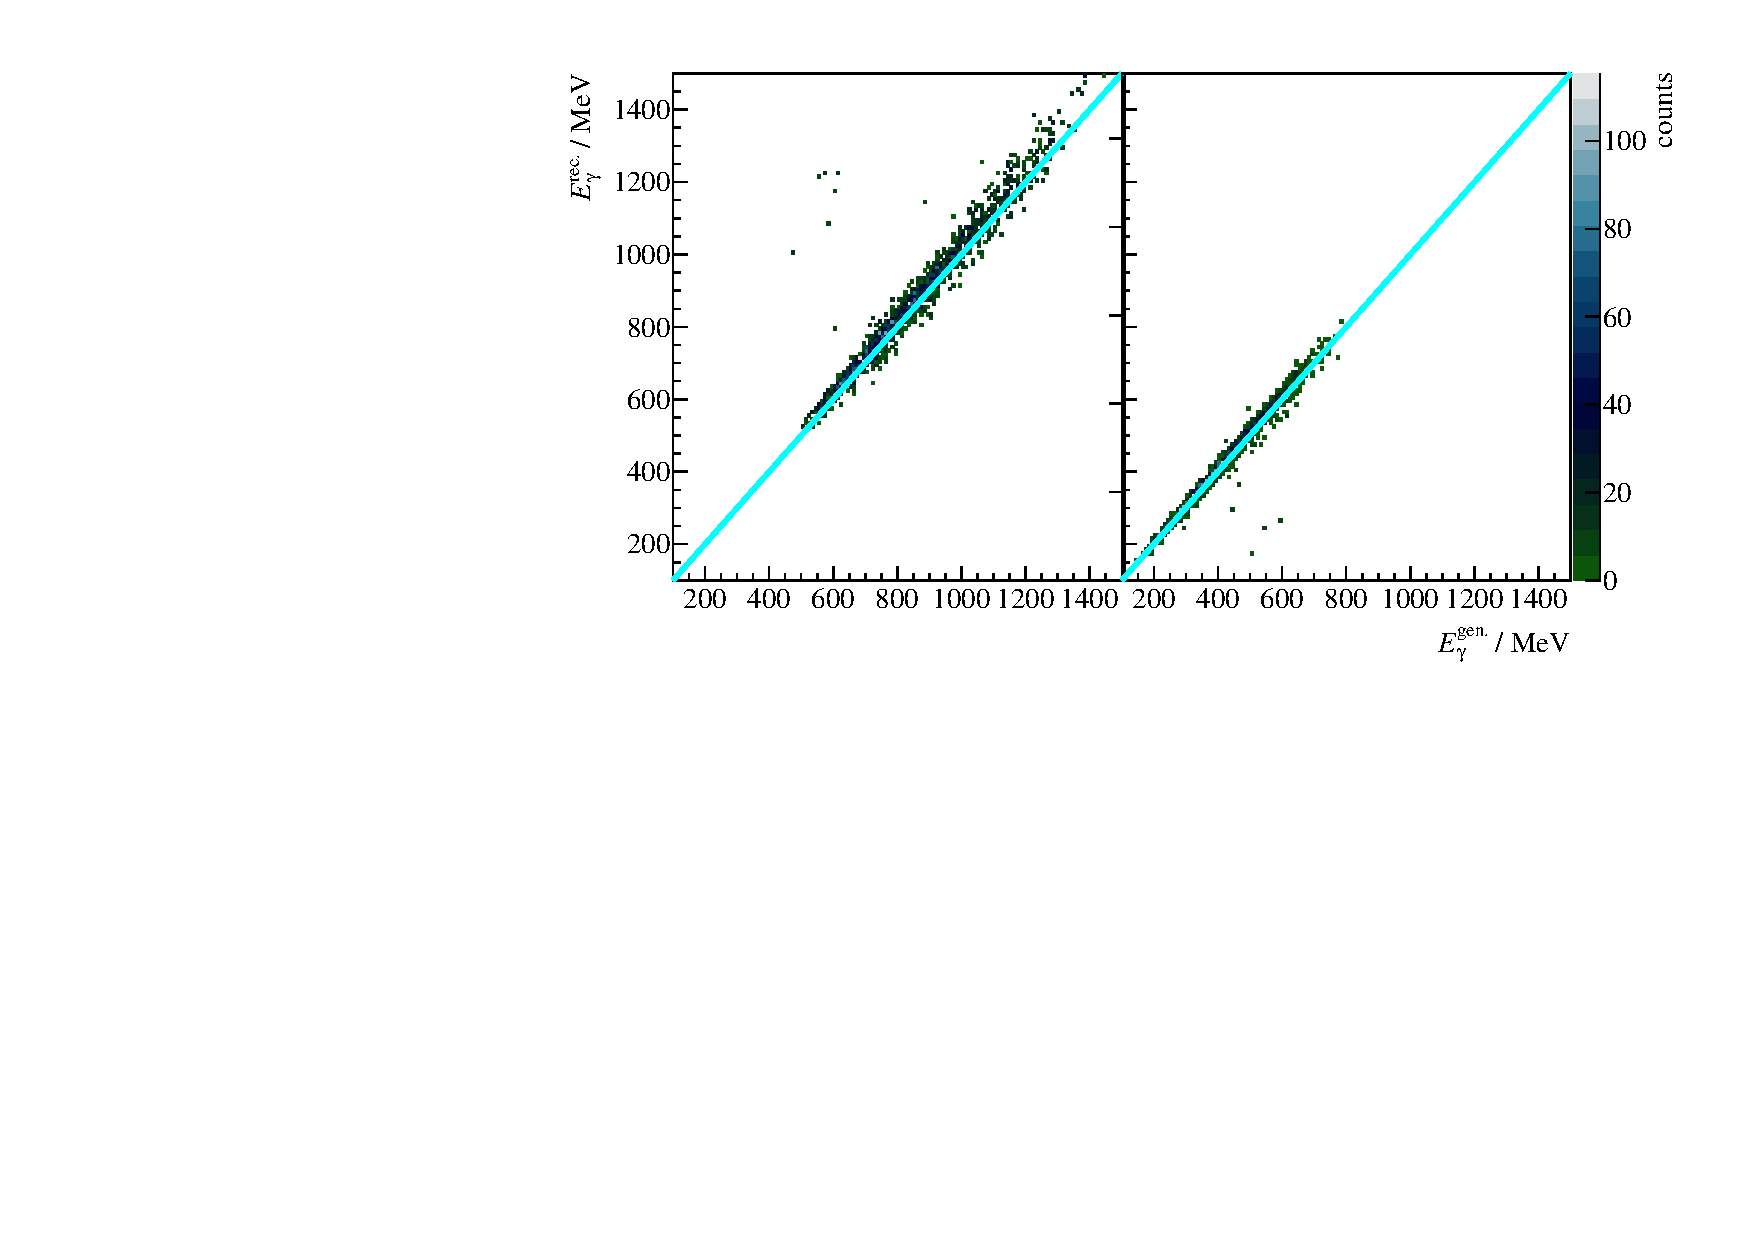
\includegraphics[width=\linewidth]{../figs/hydrogen/2pi0_gammas.pdf}
	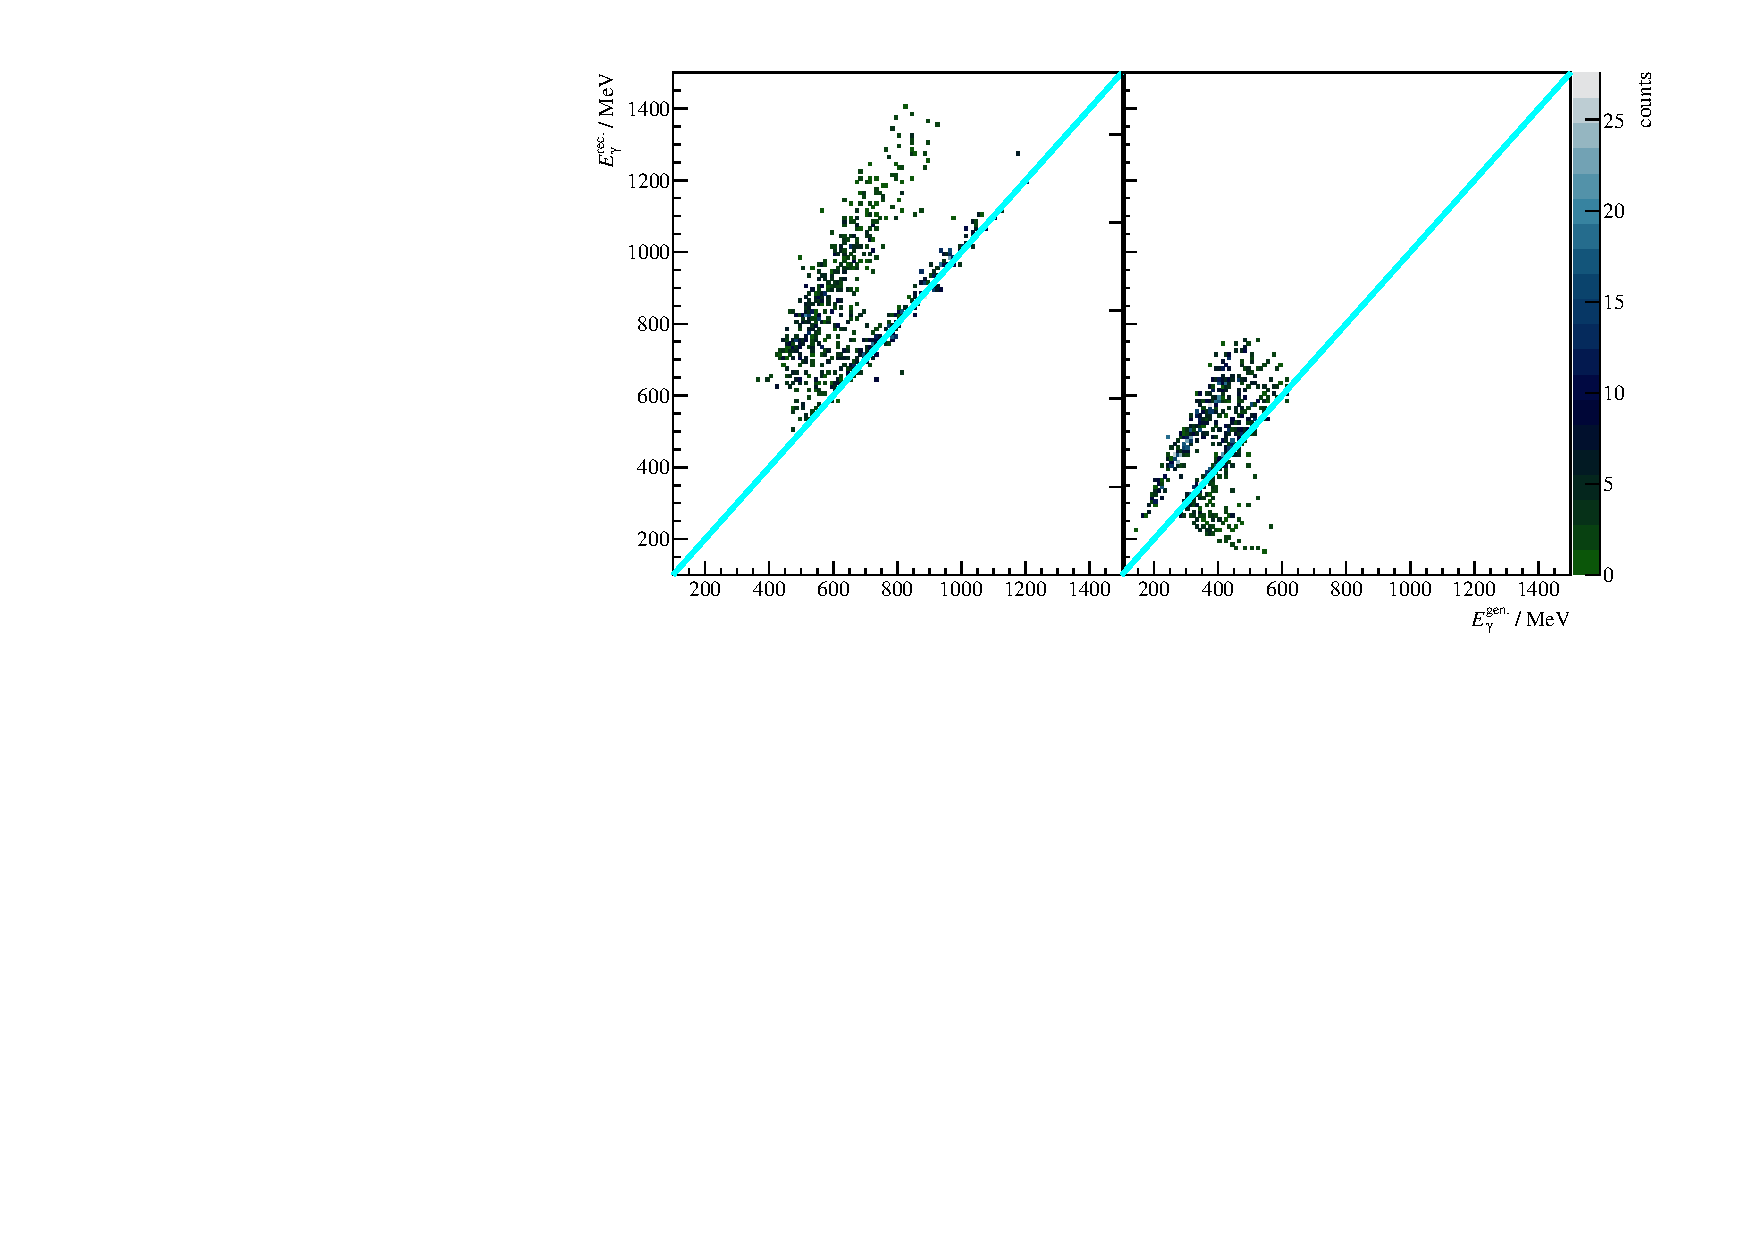
\includegraphics[width=\linewidth]{../figs/hydrogen/pi0eta_gammas.pdf}
 	\caption{$E_\gamma^\text{gen}$ vs. $E_\gamma^\text{rec}$ of $\gamma_1$ and $\gamma_2$ for $2\pi^0$ (top) and $\pi^0\eta$ (bottom) production. The slope $E_\gamma^\text{gen}=E_\gamma^\text{rec}$ is marked by a solid line.}
 	\label{fig:mcgenvsrec}
 \end{figure}
Energies that are correctly reconstructed lie on the slope of $E_\gamma^\text{gen}=E_\gamma^\text{rec}$, which is the case for nearly all events of $2\pi^0$ production. However for $\pi^0\eta$ reactions a sizable amount of events lies offside the slope towards higher reconstructed energies. This indicates on one hand that in $2\pi^0$ production, the energies of  $\gamma_3$ and $\gamma_4$ nearly always do not surpass the reconstruction threshold and on the other hand that photons with an energy above threshold may still be lost during reconstruction because they are falsely combined to one cluster with either $\gamma_1$ or $\gamma_2$ resulting in too large reconstructed energies. Too small reconstructed energies are also observed beacause energy may get los in insensitve detectro materials. Figure \ref{fig:mcangle} shows the polar angle difference between $\gamma_3$ and $\gamma_2$ of the MC $\pi^0\eta$ final state which clearly peaks centered at small angles, explaining why the false combination of two photons may happen during reconstruction.
\begin{figure}[htbp]
	\centering
	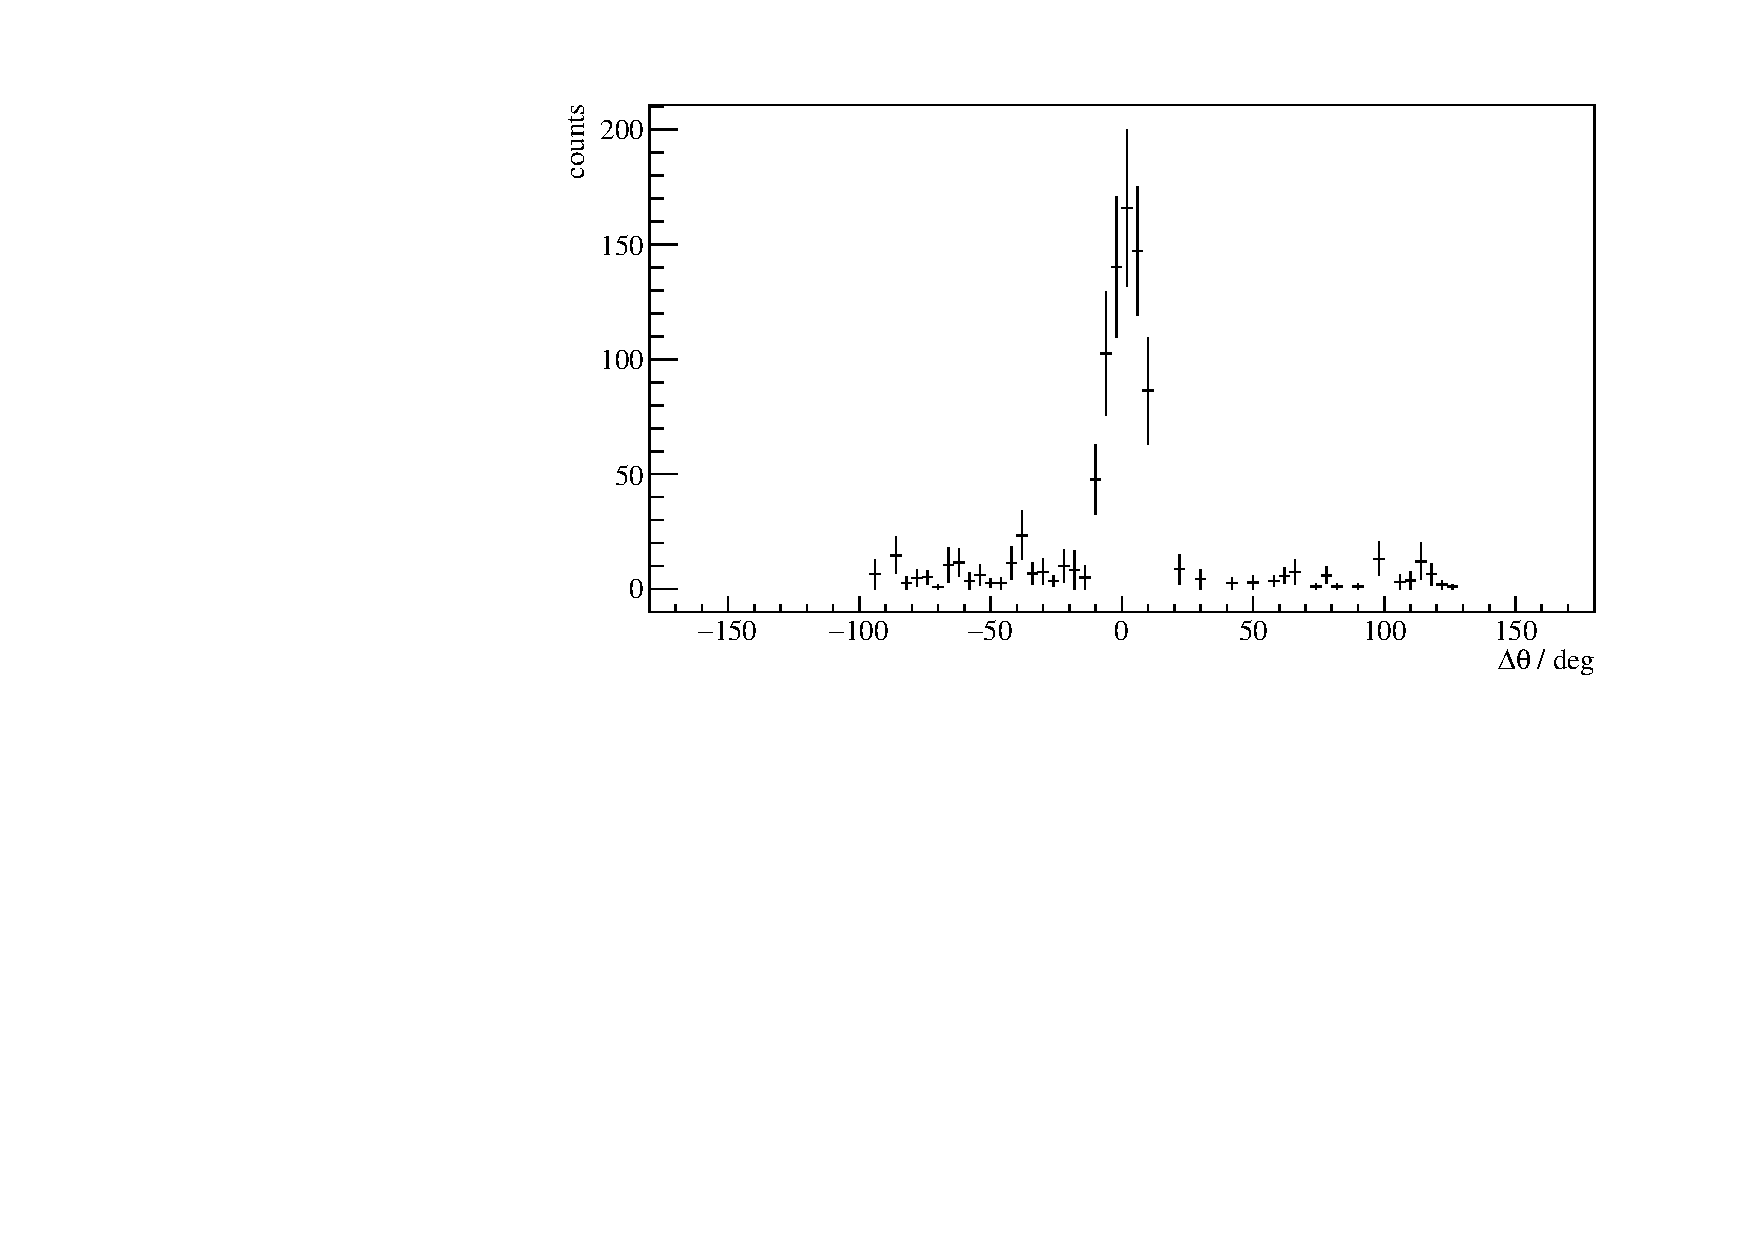
\includegraphics[width=\linewidth]{../figs/hydrogen/mcgammas_td_pi0eta.pdf}
	\caption{Polar angle difference $\Delta\theta$ between $\gamma_2$ and $\gamma_3$ of the $\pi^0\eta$ final state.}
	\label{fig:mcangle}
\end{figure}
Similar results are found with $2\pi^0$ production events but less distinct. It is evident that neither the two lost photons, nor the two reconstructed photons are correlated, i.e. decay products of the same meson ($\pi^0,\eta$).

Considering the above one can now say that $2\pi^0$ and $\pi^0\eta$ events pass the $\eta'$ event selection because 
\begin{enumerate}
	\item two uncorrelated low energy photons are lost during reconstruction and the remaining two pass the kinematic cuts by chance, since they too are uncorrelated (see figure \ref{fig:mcgammas1}),

	\item one low energy photon is lost. Two of the remaining three photons are combined to one in favor of the higher energetic photon since they were emitted in the same direction. The two reconstructed photons are uncorrelated and pass the event selection randomly, as shown in figure \ref{fig:mcgammas2}.
\end{enumerate} 
	\begin{figure}[htbp]
	\centering
	\begin{subfigure}{.49\linewidth}
		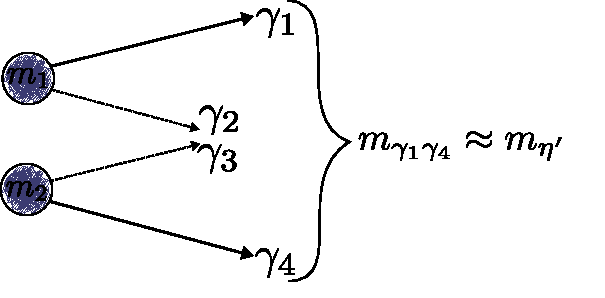
\includegraphics[width=\linewidth]{../figs/inkscape/mcgammas1.pdf}
		\subcaption{Two photons get lost while the remaining two get falsely combined to form a $\eta'$ meson\\}
		\label{fig:mcgammas1}
	\end{subfigure}
	\begin{subfigure}{.49\linewidth}
		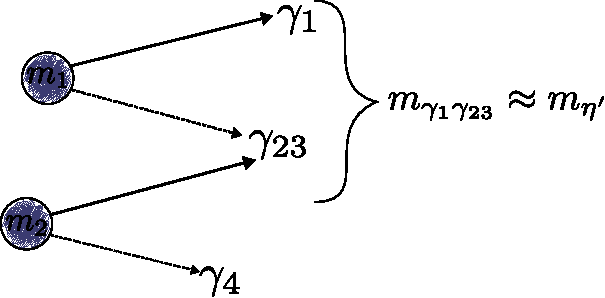
\includegraphics[width=\linewidth]{../figs/inkscape/mcgammas2.pdf}
		\subcaption{One photon gets lost, in addition two photons are grouped as one. The remaining two get falsely combined to form a $\eta'$ meson}
		\label{fig:mcgammas2}
	\end{subfigure}
	\caption{Illustration of the misidentification process during reconstruction. Enumeration of photons is now arbitrary.}

\end{figure}
These claims are indeed further validated if one examines the polar angle that is reconstructed from the falsely assigned $\eta'$ candidates using the surviving two photon momenta. This can be compared to the generated polar angle that is built using all four final state photon momenta in the CMS $\mathbf{p}_{\gamma_i}$. They add up to the artificial two-meson momentum $\mathbf{p}_m$ which in the CMS has the same magnitude but opposite direction as the recoil proton with momentum $\mathbf{p}_\text{recoil}$
$$
	\mathbf{p}_m=\sum_{i=1}^4\mathbf{p}_{\gamma_i}=-\mathbf{p}_\text{recoil}.
$$ If the lost photons have very low energies and/or are emitted in the same direction as other photons one would expect the polar angle that is spanned by the four final state photons approximately agrees with the polar angle that is built using the two photons that survived event selection, such that $\cos\theta(4\gamma)\approx\cos\theta(2\gamma)$. This is exactly what is observed, as figure \ref{fig:mccostheta} shows for both background reactions: the generated CMS angle $\cos\theta_\text{gen.}$ is plotted against the reconstructed CMS angle $\cos\theta_\text{rec.}$. The events are clearly distributed around the slope $\cos\theta_\text{gen.}=\cos\theta_\text{rec.}$ which is indicated by the solid line. This is an important result for the later analysis: if the background contributions are taken into account quantitatively then the extracted beam asymmetry has to be corrected by the asymmetry stemming from background reactions. This is only possible if the background reactions from e.g. $2\pi^0$ events realize the same bins in beam energy and CMS angle as in a dedicated measurement of the beam asymmetry in the respective photoproduction reaction. 
\begin{figure}[htbp]
	\centering
	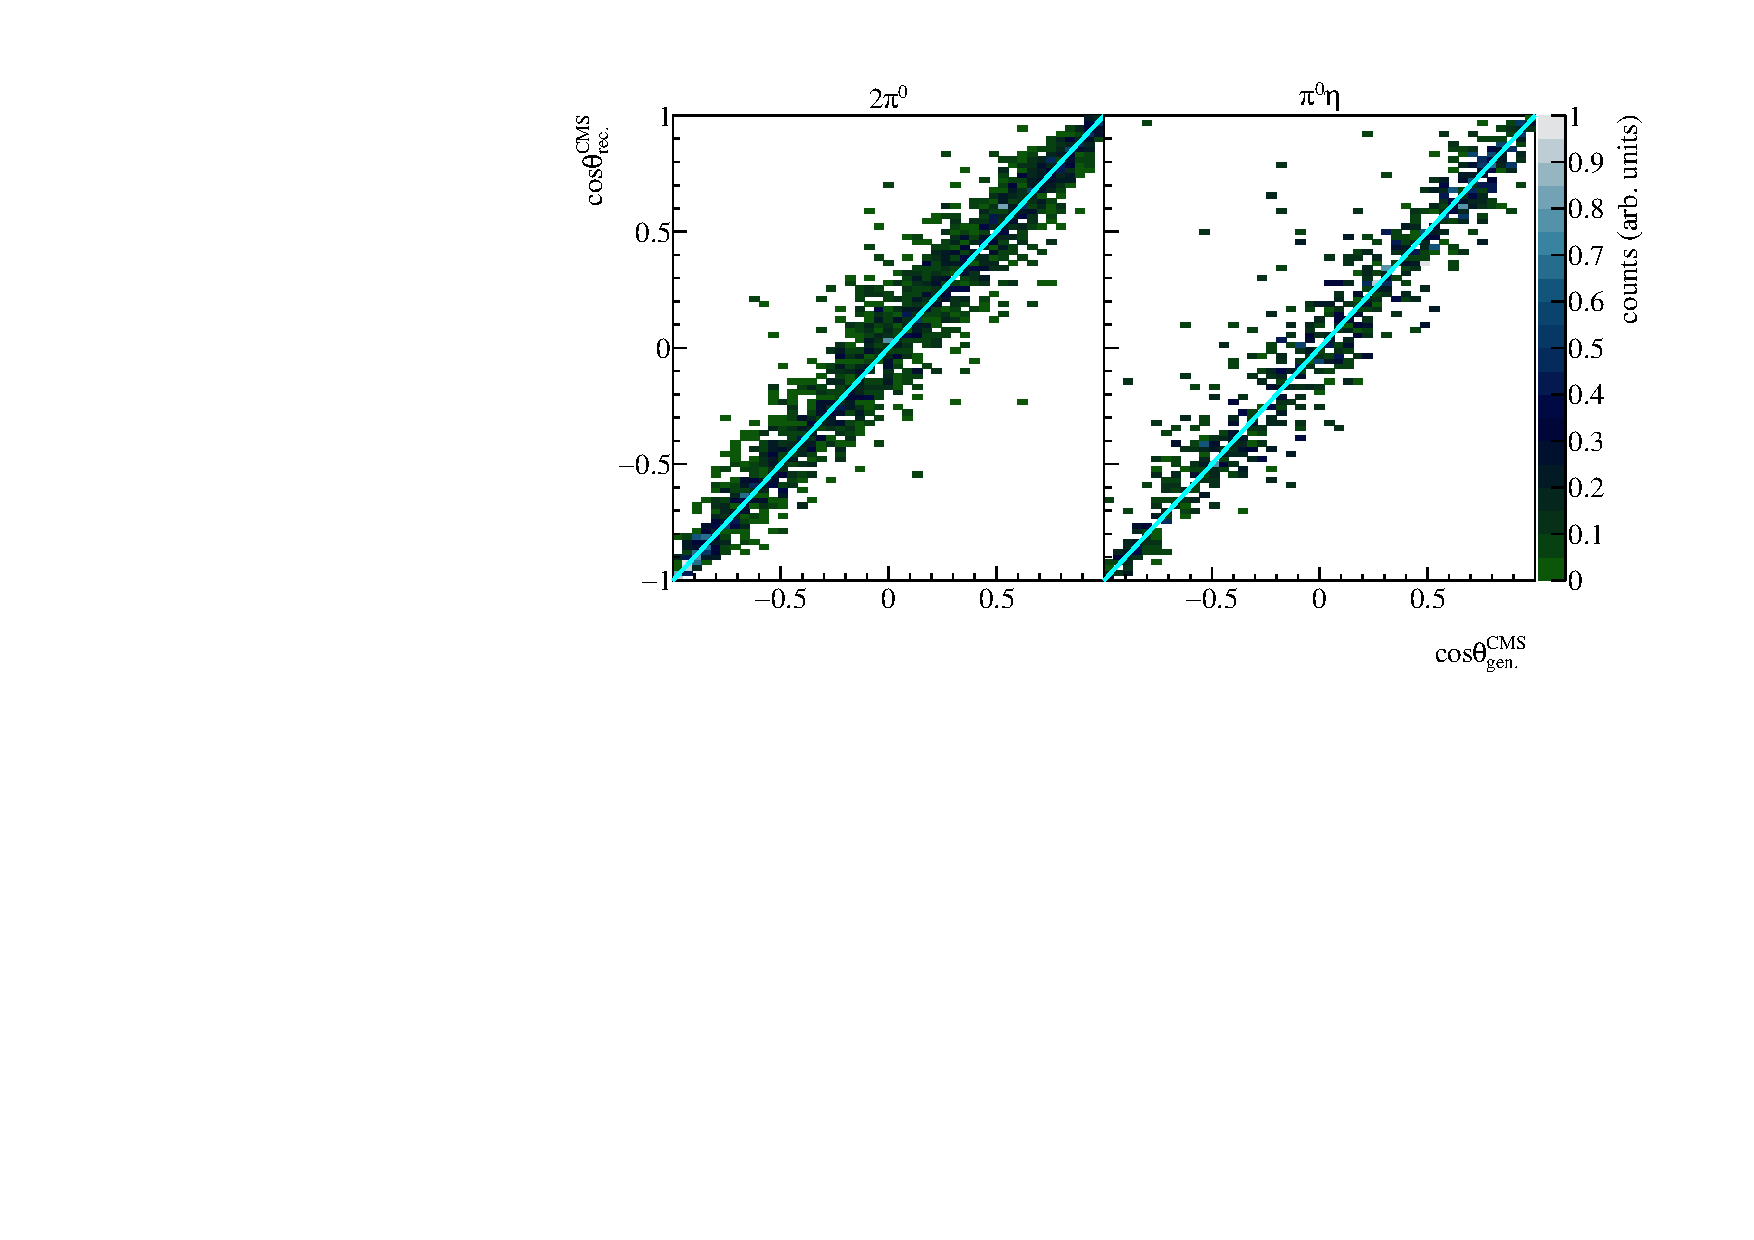
\includegraphics[width=\linewidth]{../figs/hydrogen/mcgammas_ct.pdf}
	\caption{Generated CMS angle $\cos\theta_\text{gen.}$ vs. reconstructed CMS angle $\cos\theta_\text{rec.}$ for both background reactions. The slope $\cos\theta_\text{gen.}=\cos\theta_\text{rec.}$ is indicated by the solid line.}
	\label{fig:mccostheta}
\end{figure}
\subsection{Examination of additional cuts}
\label{subsec:addcuts}
Since the background contributions are significantly beyond a neglible amount it would be desirable to remove them through additional cuts that at the same time do not remove too many signal events. However, this proved to be a complicated task because the background reactions are reconstructed from real photons which happen to be in the $\eta'$ invariant mass range. Therefore they are not distinguishable from $\eta'\to\gamma\gamma$ photons in terms of energy, momentum (direction) or created clustersize in the calorimeter crystals. The false combination of two photons into one cluster also is not observable as such since the impact of one photon with energy $E$ may create a cluster with clustersize $C$ which at the same time can be created by two photons in the same direction with energies $E_1+E_2=E$ and clustersizes $C_1+C_2=C$. Thus, to find any characteristics that separate background from signal events, one has to analyze properties of either the recoil proton or the reaction kinematics as a whole.
\subsubsection{Proton cut}
Very close to the $\eta'$ production threshold, the meson system is not boosted very often in forward direction as long as real $\eta'$ mesons are produced. As a consequence the recoil proton may escape to very forward angles in the lab system which corresponds to the proton being detected in the MiniTAPS calorimeter. Falsely reconstructed $2\pi^0$ or $\pi^0\eta$ events have lower production thresholds such that the mesons will be boosted forward and the recoil proton is detected rather in the foward detector or the Crystal Barrel calorimeter. Figure \ref{fig:p_det} shows for the two energy bins (starting at \SI{1400}{\mega\eV}) the detector that was hit by the recoil proton for $\eta', 2\pi^0$ and $\pi^0\eta$ MC data. At threshold nearly all protons of $\eta'$ events are detected in the MiniTAPS calorimeter while this is only the case for $57\%$ of $2\pi^0$ events and $20\%$ of $\pi^0\eta$ events. Towards higher energies this distribution along detectors smears out and is approximately equal for all reactions. Yet, not enough statistics  are collected in the energy bin close to threshold for a cut based on the proton detector hit to have significant signal, as this bin contains less than 7\% of total $\eta'$ candidates. The poor statistics in this bin also make determining background from MC fits difficult. Thus, as has been mentioned before, the energy bin from \SIrange{1400}{1500}{\mega\eV} was not included in the analysis. Consequently no cut based on proton detector hits could be applied to the remaining data. Apart from directional information near threshold protons from signal and background events could not be distinguished.
\begin{figure}[htbp]
	\centering
	\begin{subfigure}{\linewidth}
			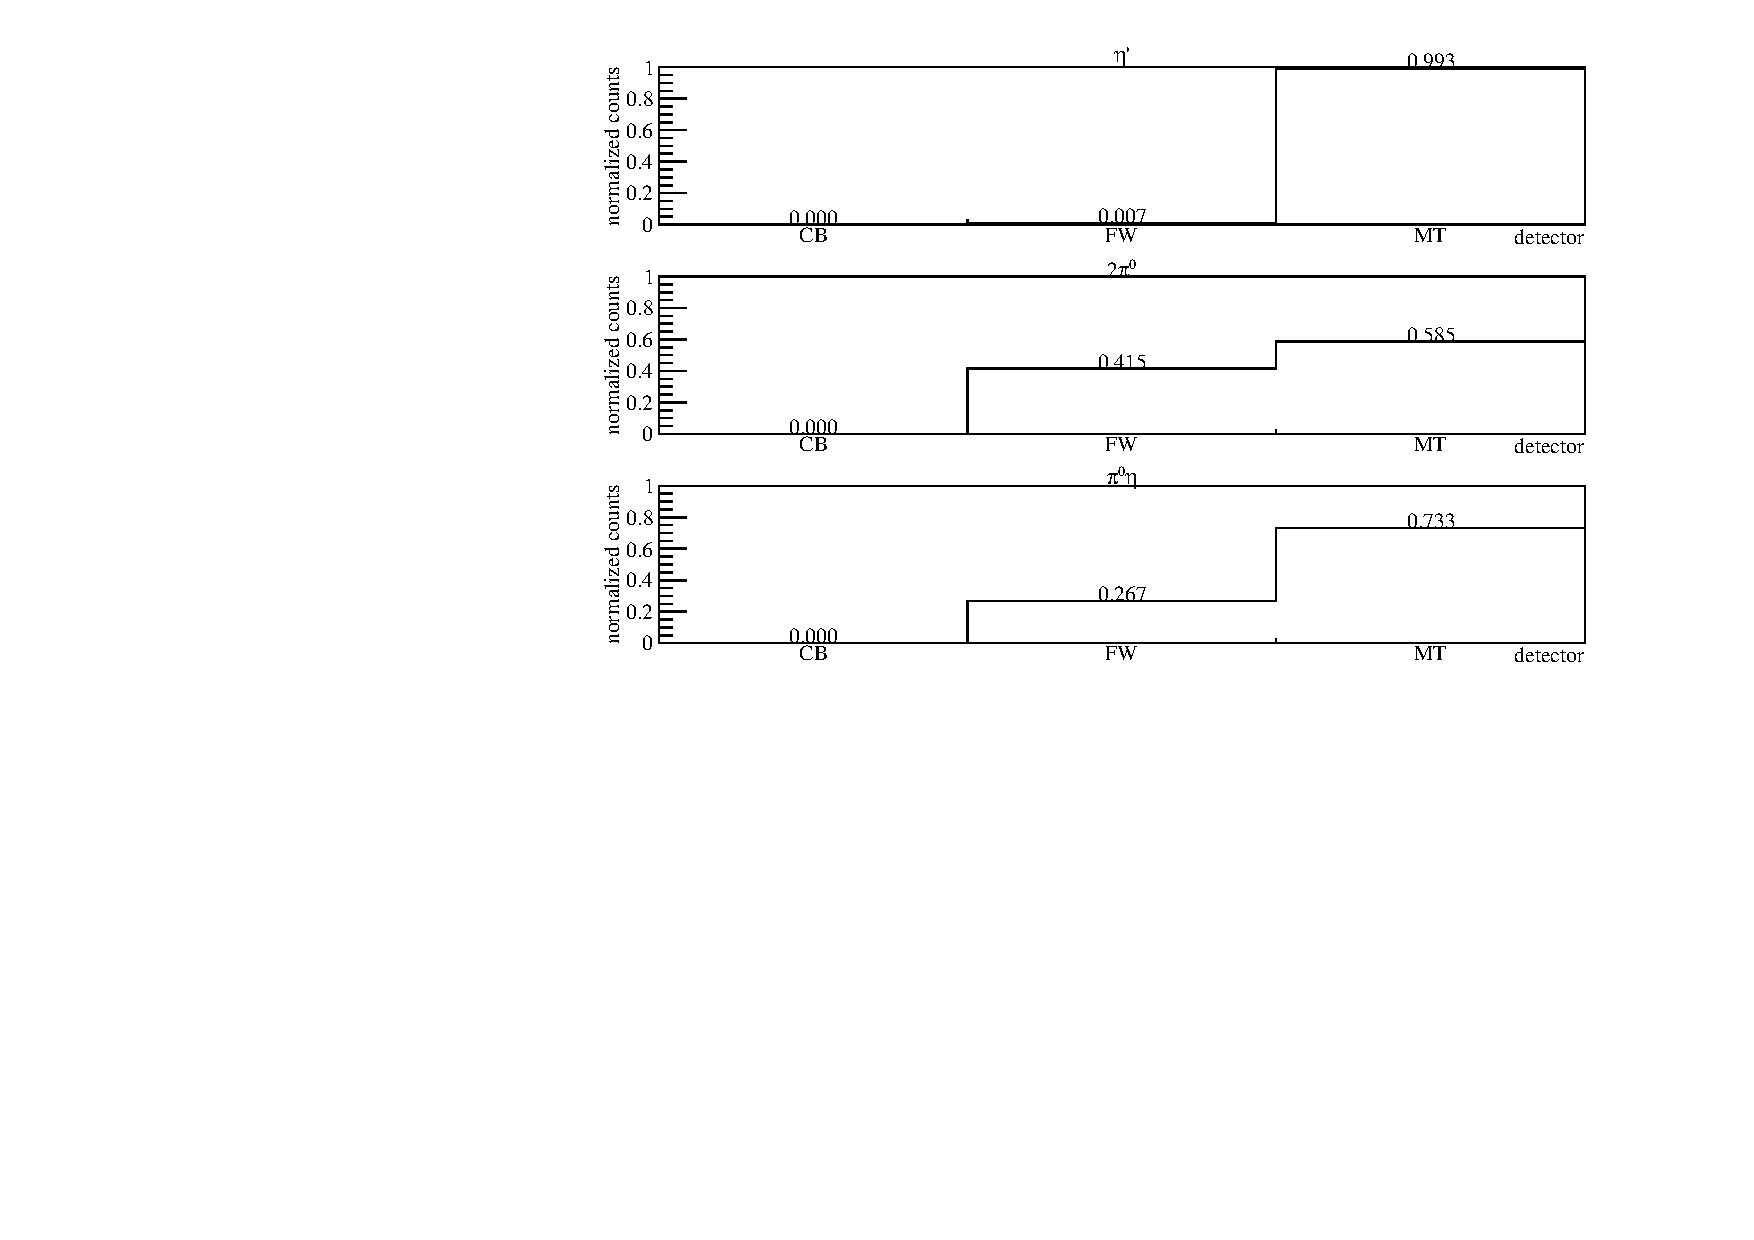
\includegraphics[width=\linewidth]{../figs/hydrogen/p_det/p_det0.pdf}
	 		\subcaption{$\SI{1400}{\mega\eV}\leq E_\gamma<\SI{1500}{\mega\eV}$}
	\end{subfigure}
	\begin{subfigure}{\linewidth}
	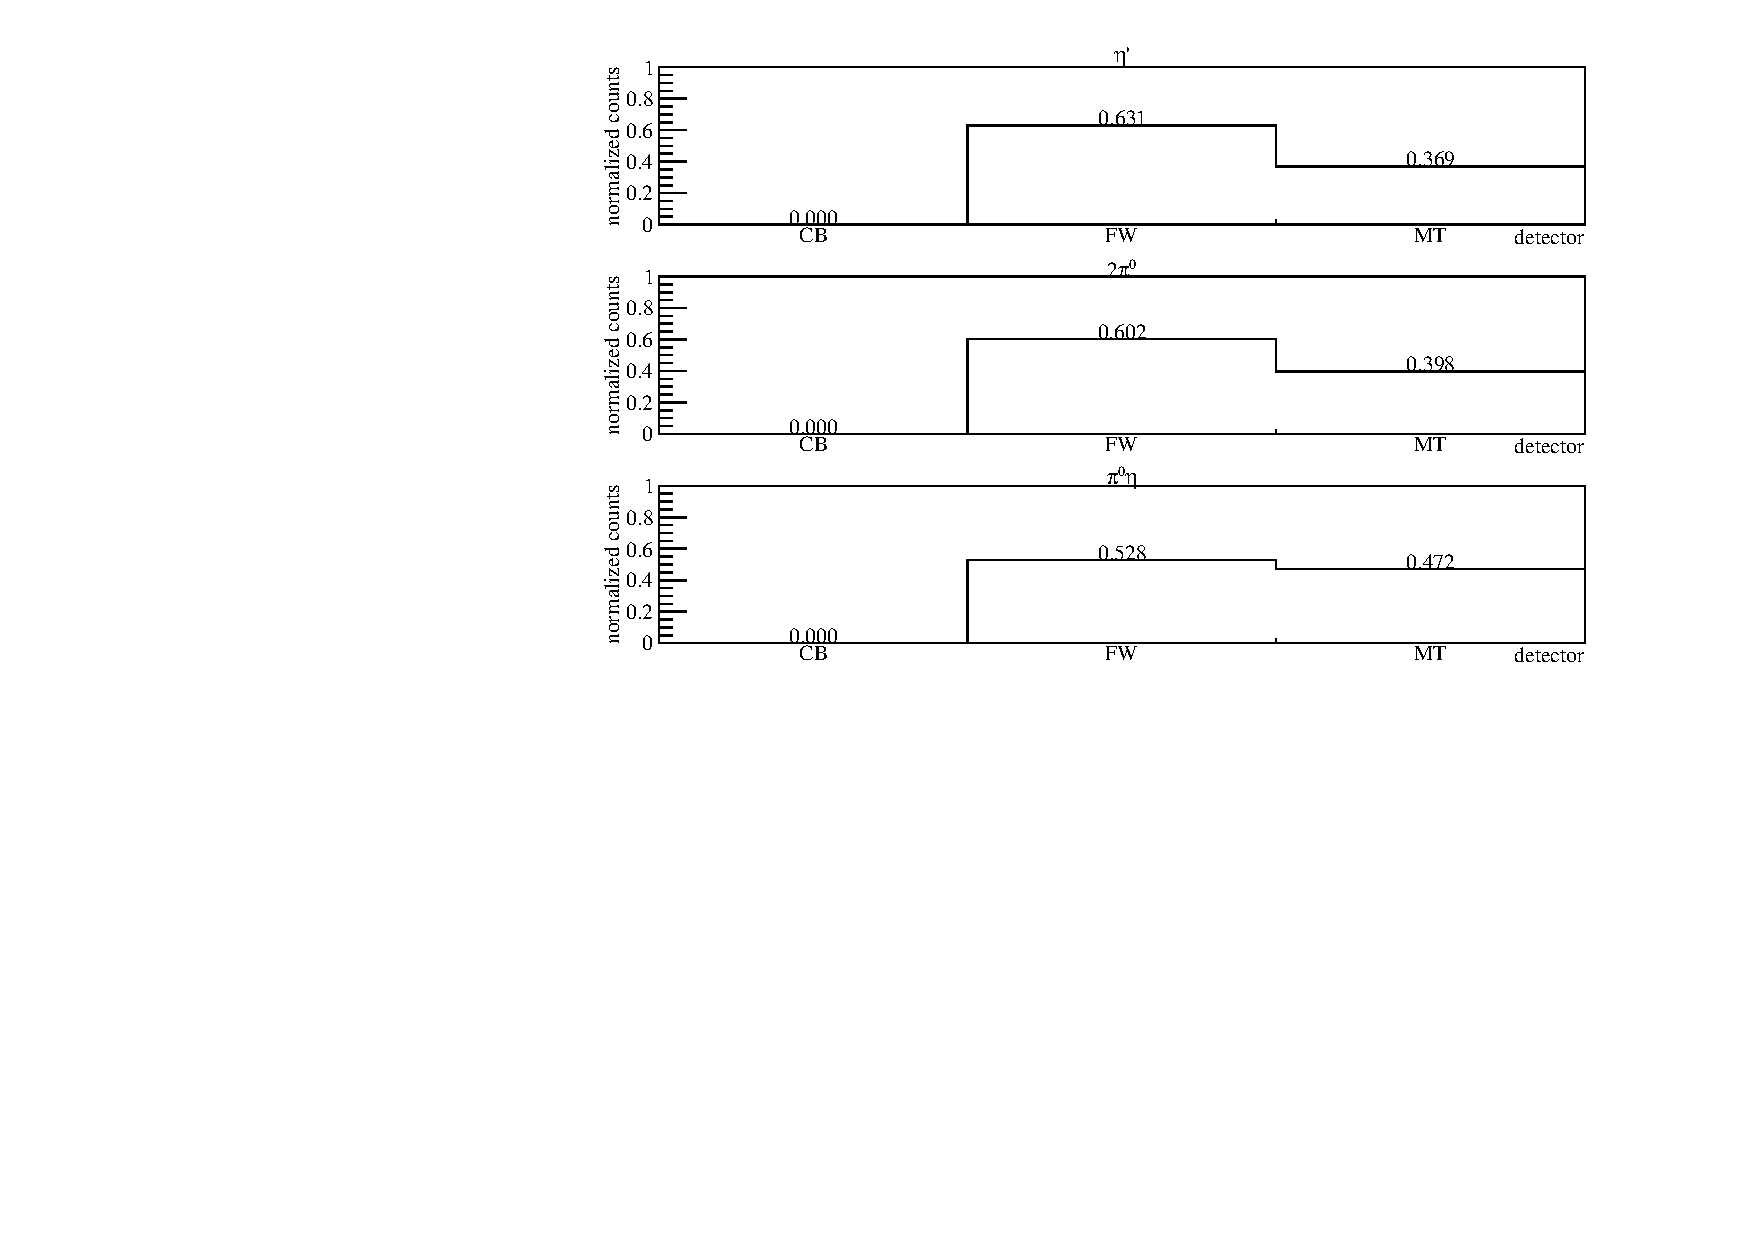
\includegraphics[width=\linewidth]{../figs/hydrogen/p_det/p_det1.pdf}
	\subcaption{$\SI{1500}{\mega\eV}\leq E_\gamma<\SI{1600}{\mega\eV}$}
\end{subfigure}

	\caption{Detector hits of the recoil proton, as obtained from MC data for the production of $\eta',2\pi^0$ and $\pi^0\eta$. CB: Crystal Barrel, FW: forward dector, MT: MiniTAPS}
	\label{fig:p_det}
	
\end{figure}
\subsubsection{Reaction kinematics}
As has been  mentioned before, the measured photoproduction reactions are in fact overdetermined, meaning that one reaction particle can be treated as missing. This can be used to calculate the beam photon energy
\begin{equation}
	E_\gamma^\text{calc}=\frac{-0.5\cdot m_{\eta'}^2+m_pE_{\eta'}}{m_p-E_{\eta}'+|p_z|_{\eta'}},
\label{eq:ebeam}
\end{equation}
where $m_p$ is the proton $m_{\eta'}$ the $\eta'$ mass, $E_{\eta'}$ is the meson energy and $|p_z|_{\eta'}$ is the meson momentum in $z$-direction. Comparing this with the measured beam energy one may tell $\eta'$ events apart from background events where mesons with smaller masses have been produced. If equation \eqref{eq:ebeam} is used to calculate the  beam energy, i.e. inserting the $\eta'$ mass, background events from reactions with smaller masses will cause smaller calculated beam energies. The difference of measured and calculated beam energy $\Delta E= E_\gamma^\text{meas}-E_\gamma^{calc}$ is shown in figure \ref{fig:beame}. The data points are shown as open circles and solid histograms represent fitted MC data where the turquoise histogram is the sum of all MC histograms. A broad peak centred slightly off 0 towards lower energy differences is visible because plugging in the literature values for $m_p$ and $m_{\eta'}$ tends to overestimate the calculated energy. It also exhibits a broad shoulder towards higher energy differences. The MC describe the data very well, consisting mainly of $\eta'$ and $2\pi^0$ MC, as expected. The $\pi^0\eta$ MC describe a flat shape. The background MC show a trend towards energy differences $>0$, as predicted by equation \eqref{eq:ebeam}. In principle the distribution of background and $\eta'$ MC now allow to introduce an upper bound on the beam energy difference rejecting any desired amount of background. However, simultaneously a significant amount of $\eta'$ events have to be discarded if this cut should have remarkable influence on the background events, as is shown in table \ref{tab:beame}. 
\begin{table}[htbp]
	\centering
	\begin{tabularx}{\linewidth}{ccYY}
		\toprule
		upper limit of $\Delta E$ / MeV& rel. loss of signal events  / \% &\multicolumn{2}{c}{relative loss of bkg. events / \%} \\
		&& $2\pi^0$ & $\pi^0\eta$\\
		\hline
		0 & 36 & 71&59\\
		50 & 21 & 53&36\\
		100& 10&33& 18\\
		150 & 4 & 15 &6\\
		
		\bottomrule
	\end{tabularx}
	\caption{Relative loss in signal and background events if a cut on $\Delta E$ is applied.}
	\label{tab:beame}
\end{table}
\noindent Considering that only 8000 $\eta'$ candidates could be extracted, any cut removing sizable fractions of signal events will have grave impact regarding the statistical error for the later analysis of the beam asymmetry. It was decided not to imply any further cuts on the data and proceed with the selected events as described previously. Because results for the beam asymmetry in $2\pi^0$ production are available \cite{mahlbergphd} it is not crucial to remove all remaining background events since the extracted beam asymmetry can be corrected proportionately, depending on the amount and type of background in a particular bin, see section \ref{sec:sigma_etap}. 
\begin{figure}[htbp]
	\centering
	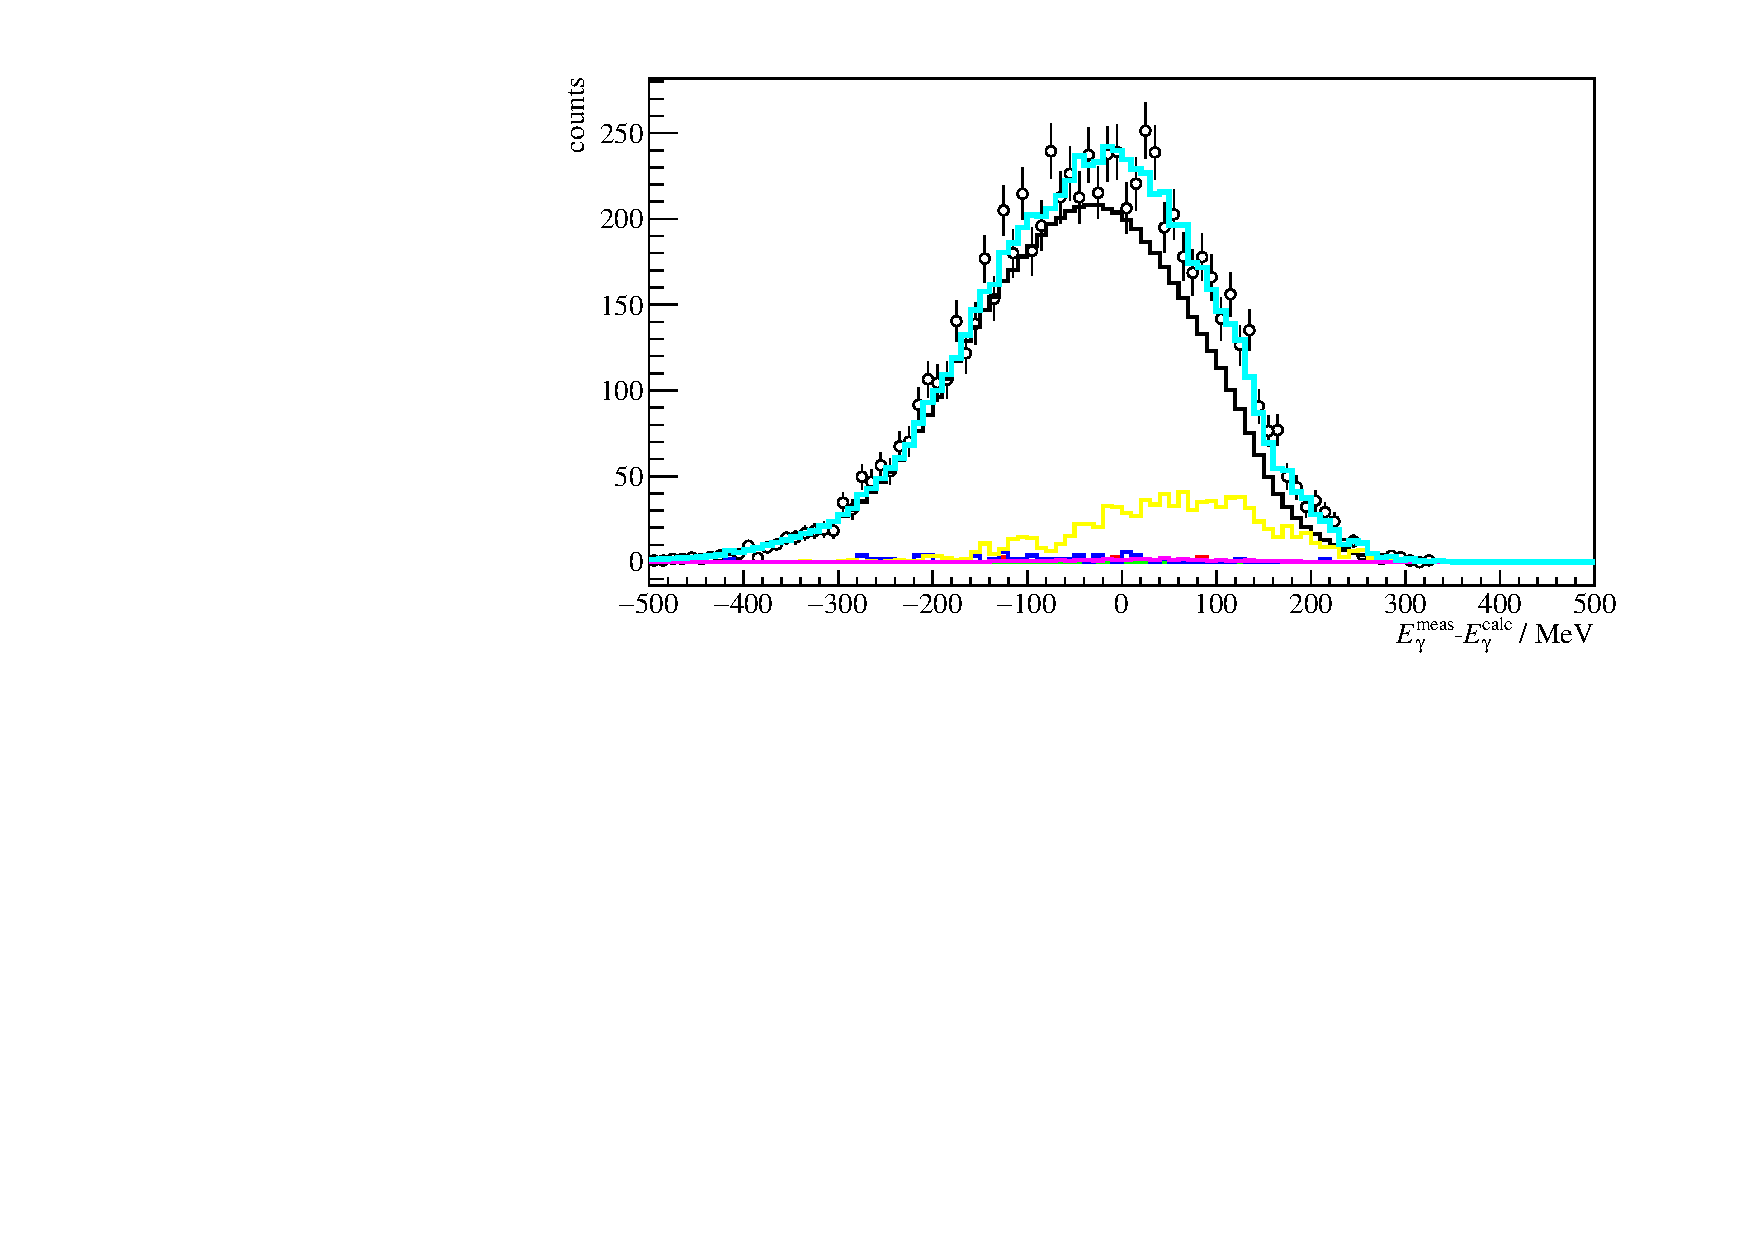
\includegraphics[width=\linewidth]{../figs/hydrogen/calc_beam.pdf}
	\caption{Difference in measured and calculated beam energy. Data points are shown as open circles, MC data as solid histograms: in black $\eta'$, in green $\pi^0$, in red $\eta$, in blue $\omega$, in yellow $2\pi^0$ and in magenta $\pi^0\eta$. The turquoise histogram is the sum of all MC histograms.}
	\label{fig:beame}
\end{figure}

\section{Summary of event selection}
\subsection{Reaction $\gamma p\to p\eta'\to p\gamma\gamma$}
The reaction $\gamma p\to p\eta'$ could be selected successfully. Combinatorial background was removed using the time information of initial and final state particles. Furthermore, the measured energies and momenta of all final state particles were utilized when applying constraints, that were derived from energy and momentum conservation, to $\gamma p\to\eta'\to\gamma\gamma$ event candidates. A significant amount of background still passes the event selection process which could be traced back to $2\pi^0$ and $\pi^0\eta$ production using Monte Carlo simulations. Very restricted possibilities to exclusively select signal from background events were found but in the end not used as they still remove sizable fractions of signal events in order to get rid of background events.

To illustrate again the impact of all applied cuts, the invariant mass summed over all angular and energy bins of the final state photons is shown again in figure \ref{fig:invm_pretty} where the spectrum can be seen after each individual cut successively. While at first only slight structures in the invariant mass spectrum can be observed, in the end a clear, peak-like structure is visible, indicating the general success of the event selection that has been described in this chapter. The signal to background ratio is improved by each applied cut where the time cut clearly removes the most (combinatorial) background. Note that there are differences of three and two orders of magnitude in statistics for $\pi^0$ or $\eta$ meson production compared to $\eta'$ production in the neutral decay channel. 
\begin{figure}[t]
	\centering
	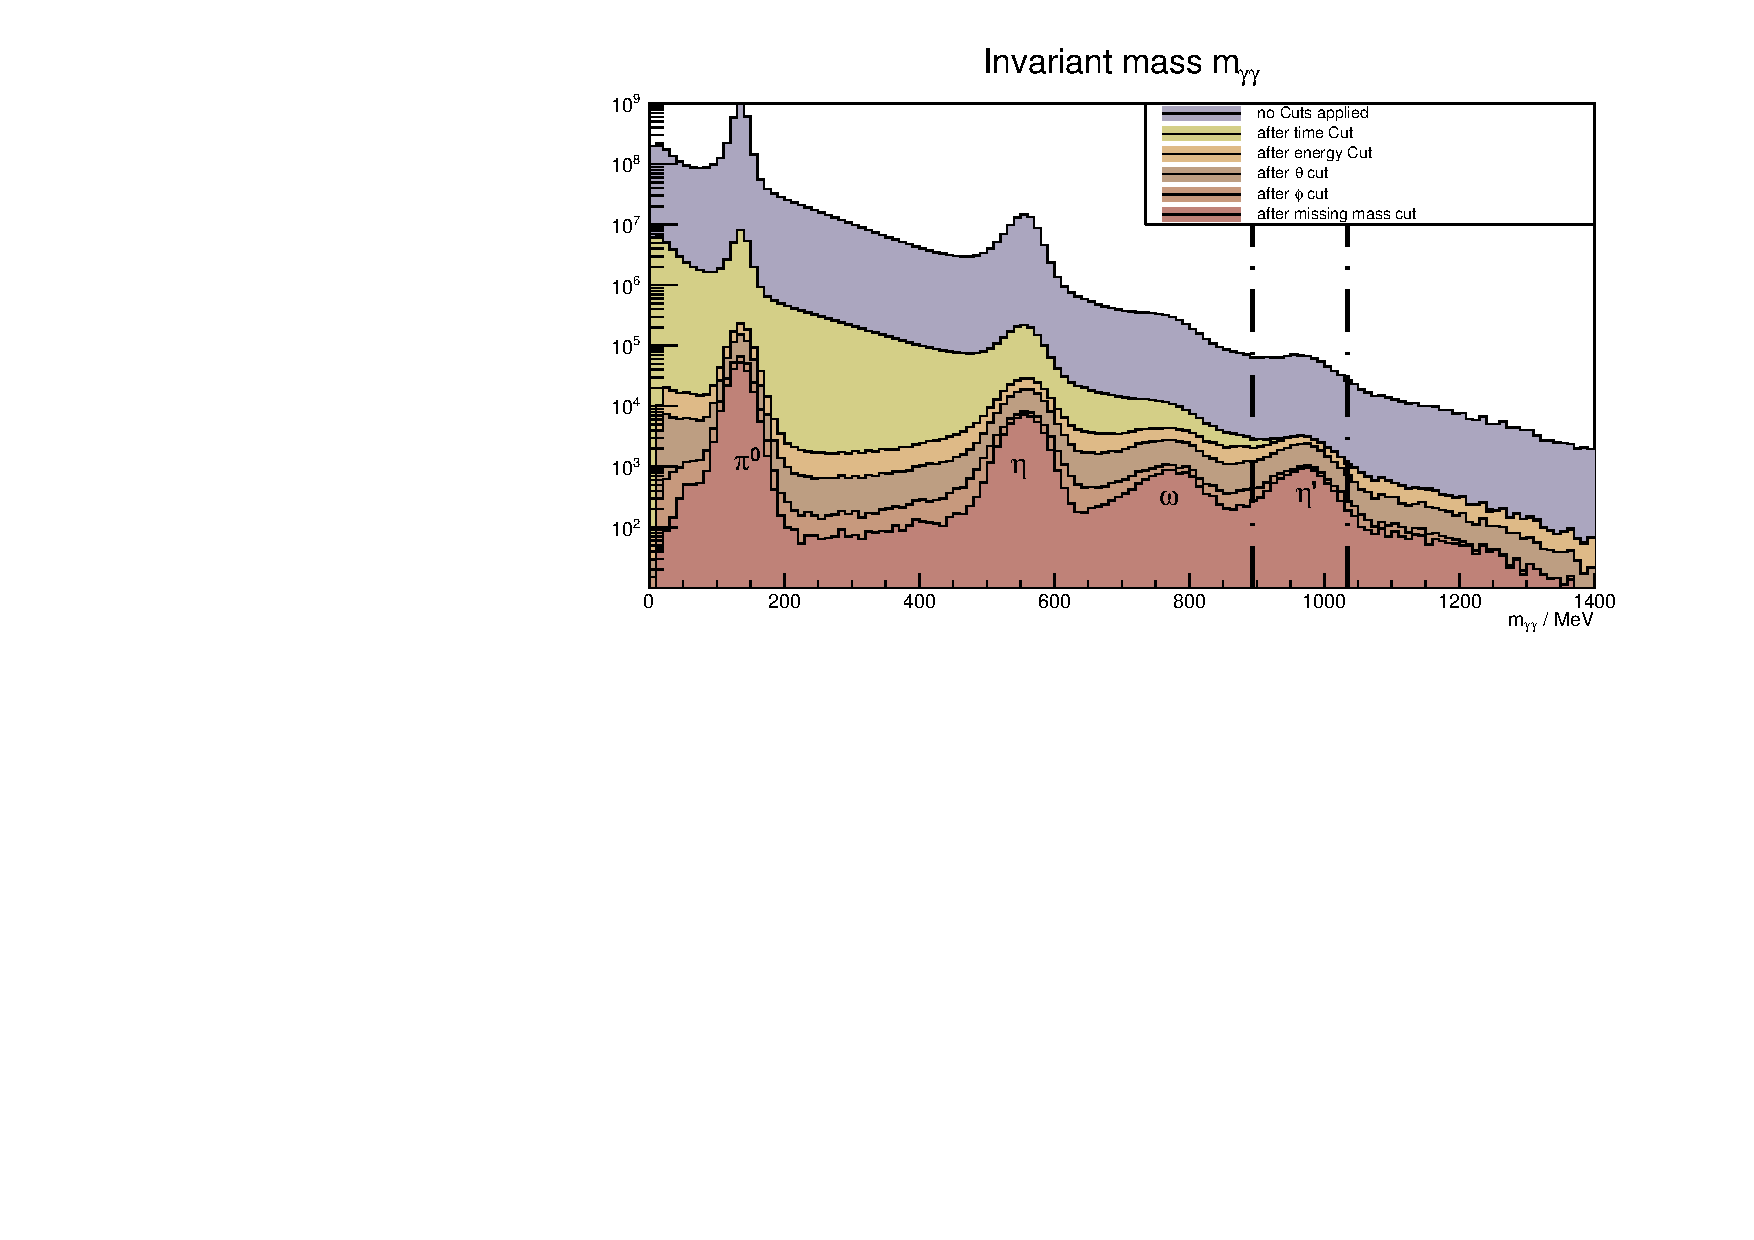
\includegraphics[width=\linewidth]{../figs/hydrogen/inv_mass_pretty.pdf}
	\caption{Invariant mass spectrum passing different stages in the event selection process. In the end clear peaks for all possibly produced mesons are visible. The vertical lines indicate the mean cut ranges over all energy and angle bins.}
	\label{fig:invm_pretty}
\end{figure}
\subsection{Reaction $\gamma p\to p\eta\to p\gamma\gamma$}
As has been mentioned in the beginning of this chapter, the reaction $\gamma p \to p\eta\to p\gamma\gamma$ was subject of the dissertation \cite{farahphd} and this thesis only uses the selected data to verify existing results with new fitting methods. A short summary of the event selection that is described in detail in reference \cite{farahphd} will be given in the following nevertheless.

Since a three particle final state was to be investigated, the data is first of all constrained to include only 2PED, 2.5PED and 3PED events. No charge cut was applied, so that always two final state particles were combined pairwise to form a meson candidate while the remaining particle (if measured) was assigned as proton candidate. As a next step coincidence of final state particles was checked in a similar fashion to section \ref{sec:time} with the exception that depending on the hit detectors different prompt peaks and sideband ranges were selected. Afterwards the discussed kinematic variables $\Delta\theta,\Delta\phi,m_X,m_\text{meson}$ were used to further filter out candidates for $\eta$ photoproduction. Hereby a binning of $\SI{60}{\mega\eV}$ in the beam energy and $1/6$ in $\cos\theta$ was chosen. With the help of Monte Carlo simulations background contributions from single $\pi^0$ production could be recognized. They could be explained by events were one final state photon is lost and the recoil proton falsely creates two tracks and according cuts to remove these events were made. In the end, less than $7\%$ background contamination was achieved in all kinematic bins. Figure \ref{fig:eta_sel} shows the invariant mass with each cut successively applied. At first only slight structures are visible, also because no charge cut is applied to the data, which increases the amount of combinatorial background. But with each cut the contributions from meson photoproduction become more distinct, indicating all in all a successful event selection.

\begin{figure}[htbp]
	\centering
	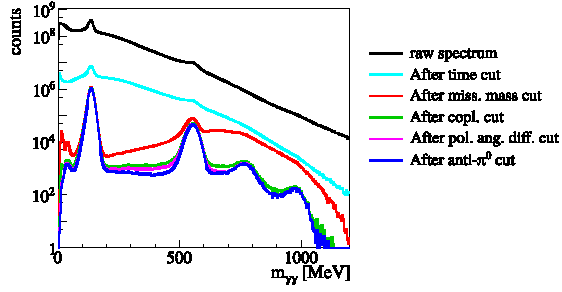
\includegraphics[width=\linewidth]{figs/eta_sel.pdf}
	\caption{Invariant mass spectrum passing different stages in the event selection process. In the end clear peaks for all possibly produced mesons are visible. Taken from \cite{farahphd}.}
	\label{fig:eta_sel}
\end{figure}
